%%% File encoding: UTF-8
%%% äöüÄÖÜß  <-- no German umlauts here? Use an UTF-8 compatible editor!

%%% Magic comments for setting the correct parameters in compatible IDEs
% !TeX encoding = utf8
% !TeX program = pdflatex 
% !TeX spellcheck = en_US
% !BIB program = biber

\RequirePackage[utf8]{inputenc} % Remove when using lualatex or xelatex!
\RequirePackage{hgbpdfa}        % Creates a PDF/A-2b compliant document

\documentclass[bachelor,english,smartquotes]{hgbthesis}
% Valid options in [..]: 
%    Type of work: 'diploma', 'master' (default), 'bachelor', 'internship' 
%    Additionally for a thesis exposé: 'proposal (for 'bachelor' and 'master')
%    Main language: 'german' (default), 'english'
%    Turn on smart quote handling: 'smartquotes'
%    APA bibliography style: 'apa'
%%%-----------------------------------------------------------------------------

\graphicspath{{images/}}  % Location of images and graphics
\logofile{logo}           % Logo file: images/logo.pdf (no logo: \logofile{})
\bibliography{references} % BibLaTeX bibliography file (references.bib)

%%%-----------------------------------------------------------------------------
\begin{document}
%%%-----------------------------------------------------------------------------

%%%-----------------------------------------------------------------------------
% Title page entries
%%%-----------------------------------------------------------------------------

\title{Angular.js vs Vue.js}
\author{Cornelia Langsenlehner, Sandra Hartlauer, Michael Nußbaumer}

\programname{Mobile Computing}

\programtype{Fachhochschul-Bachelorstudiengang} % select/edit
%\programtype{Fachhochschul-Masterstudiengang}

\placeofstudy{Hagenberg}
\dateofsubmission{2024}{05}{22} % {YYYY}{MM}{DD}

\advisor{FH-Prof. Dr-Ing. Krösche Jens} % optional

%\strictlicense % restrictive license instead of Creative Commons (discouraged!)

%%%-----------------------------------------------------------------------------
\frontmatter                                   % Front part (roman page numbers)
%%%-----------------------------------------------------------------------------

\maketitle
\tableofcontents

\chapter{Preface} % German: Vorwort

This is version \textbf{\hgbDate} of the \latex document template for various
theses at the School of Informatics, Communication and Media at the University
of Applied Sciences Upper Austria in Hagenberg. We are pleased to learn that this
document collection is meanwhile also used at various other institutions in Austria
and abroad.

The document was initially created in response to requests from students after
the 2000/01 academic year when an official \latex introductory course was
offered in Hagenberg for the first time. The fundamental idea was to
"simply" convert the already existing \emph{Microsoft Word} template for
diploma theses to \latex\ and possibly to add some unique features. This quickly
turned out to be not very useful since \latex, especially concerning the
handling of literature and graphics, requires a substantially different way of
working. The result is--- rewritten from scratch and much more extensive than
the previous document---a manual for writing with \latex, supplemented with
additional (meanwhile removed) hints for \emph{Word} users. Technical details
of the current version can be found in Appendix.
%\ref{app:TechnicalDetails}.

While this document was initially intended exclusively for the preparation
of diploma theses, it now also covers \emph{master theses},
\emph{bachelor theses}, and \emph{internship reports}. The differences between
these documents have been deliberately kept small.


When creating this template, an attempt was made to work with the basic
functionality of \latex and---as far as possible---to achieve this without
additional packages. This was only partially successful; several supplementary
"packages" are necessary, but only common extensions have been used. Of course,
there is a large number of additional packages which can be helpful for further
improvements and refinements. Everyone is encouraged to experiment with these as
soon as they have the necessary self-confidence and sufficient time to
experiment. Many details and tricks are not explicitly mentioned in this
document but can be explored in the underlying source code at any time.

Numerous colleagues have provided valuable support through careful proofreading
and constructive suggestions for improvement. We thank Heinz Dobler for
consistently improving our "computer slang" and Elisabeth Mitterbauer for her
proven "orthographic eye".

Usage of this template is free without any restrictions and not bound to any
mention. However, when used as a basis for one's work, one should not simply
start working on it, but at least \emph{read} the essential parts of the
document and, if possible, take them to heart. Experience has shown that this
improves the quality of the results significantly.

This document and the associated \latex classes have been available since
November 2017 on CTAN%
\footnote{Comprehensive TeX Archive Network} 
as package \texttt{hagenberg-thesis},
%
\begin{itemize}
	\item[]\url{https://ctan.org/pkg/hagenberg-thesis}.
\end{itemize}
%
The current source code, as well as additional materials---such as a wiki with
instructions for the integration of often requested functionalities and
extensions---can be found at
%
\begin{itemize}
  \item[]\url{https://github.com/Digital-Media/HagenbergThesis}.%
  \footnote{\url{https://github.com/Digital-Media/HagenbergThesis/blob/main/CHANGELOG.md}
  contains a list of chronological changes (formerly included in the appendix
  of this document).}
\end{itemize}

\noindent
Despite great efforts, a document like this always contains errors and
shortcomings. Comments, suggestions, and helpful additions are welcome.
Ideally, as comments or issues on GitHub.

By the way, here, in the preface (which is common in diploma and master theses
but dispensable for bachelor's theses), you may briefly describe the genesis of
the document. This is also the place for any acknowledgments (\eg, to the
supervisor, the examiner, the family, the dog, \etc) as well as dedications and
philosophical remarks. These should be balanced and limited to a maximum of two
pages.

\vspace{6ex}
\noindent
W.\ Burger (em.) and W.\ Hochleitner\\[1ex]
University of Applied Sciences Upper Austria\\ 
Department of Digital Media, Hagenberg\\
\url{https://www.fh-ooe.at/campus-hagenberg/}
 % A preface is optional
\chapter{Abstract}

Here goes an abstract of the work, with a maximum of 1 page. Unlike other
chapters, the abstract is usually not divided into sections and subsections.
Footnotes are also not used here.

By the way, abstracts are often included in literature databases with the author
and title of the work. It is, therefore, essential to ensure that the
information in the abstract is coherent and complete in itself (\ie, without
other parts of the work). In particular, \emph{no literature references} are
typically used at this point (as is the case also in the \emph{title} of the
thesis and the German \emph{Kurzfassung})!
If such is needed---for example, because the paper is a further development of a
particular, earlier publication---then \emph{full} references are necessary for the
abstract itself, \eg, [\textsc{Zobel} J.: \textit{Writing for Computer Science
-- The Art of Effective Commu\-nica\-tion}. Springer, Singapore, 1997].

It should also be noted that special characters or list items are usually lost
when records are added to a database. The same applies, of course, to the German
\emph{Kurzfassung}.

In terms of content, the abstract should not be a list of the individual
chapters (the introduction chapter is intended for this purpose). However, it
should provide the reader with a concise summary of your thesis.
Therefore, the structure used here is necessarily different from that used in
the introduction.

\chapter{Kurzfassung}

\begin{german} %switch to German language rules
	Dies sollte eine maximal 1-seitige Zusammenfassung Ihrer Arbeit in deutscher
	Sprache sein.
	%here goes the rest of the Kurzfassung...
\end{german}

The German "Kurzfassung" should contain the same content as the English abstract.
Therefore, try to translate the abstract precisely but not word for word. When
translating, remember that certain idioms from English have no counterpart in
German or must be formulated differently. Also, word order in German is very
different from English. Without
knowledge of the German language, it is acceptable to resort to translators.
Nevertheless, hiring a skillful person for proofreading is recommended
even with the highest confidence in one's German knowledge.

The correct translation for "diploma thesis" is \emph{Diplomarbeit}, a "master
thesis" is called \emph{Masterarbeit}. For "bachelor's thesis",
\emph{Bachelorarbeit} is the appropriate translation.

By the way, for this section, the \emph{language setting} in \latex\ should be
switched from English to German to get the correct form of hyphenation. However,
the correct quotation marks must be set manually.


%%%-----------------------------------------------------------------------------
\mainmatter                                    % Main part (arabic page numbers)
%%%-----------------------------------------------------------------------------

\chapter{Introduction}
\label{cha:Introduction}


\section{Motivation}
The increasing importance of web applications in the modern digital landscape motivates this analysis. According to the UNCTAD Digital Economy Report (2019), businesses and services are rapidly moving online, which increases the demand for efficient, user-friendly, and powerful web applications. The ability of web applications to operate across various platforms allows developers to serve a wide user base without the need to develop separate applications for each operating system or device~\cite{unctad}.

\section{Challenges}

%\subsection{Hardware Platforms}
Web application development necessitates compatibility across multiple hardware platforms, including desktop computers, laptops, tablets, and mobile devices. Mao (2014) identifies the primary challenge as maintaining consistent performance and efficiency across these diverse devices~\cite{mao2014developing}.

%\subsection{Frameworks}
Additionally, the selection and management of development frameworks significantly influence the efficiency and scalability of web applications. Verma (2022) points out that different frameworks exhibit unique strengths and weaknesses concerning performance, maintainability, and user-friendliness. Verma (2022) also stresses the importance of evaluation methods in assessing the performance, security, and user-friendliness of web applications. These evaluations typically include benchmarks, test scenarios, and other empirical methods aimed at verifying the quality of the application~\cite{verma2022comparison}.

\section{Goals}
This analysis aims to provide a brief overview of both frameworks and serve as a decision-making guide by offering valuable insights into the strengths and weaknesses of both technologies. 
These insights assist development teams in making informed decisions about the most suitable technologies for specific application requirements. Additionally, they help identify optimization opportunities to continuously enhance user experience and improve development efficiency.

\section{Structure}
Besides the structure, the motivation section also covers the challenges and goals of this study. The following three chapters include the theoretical background, which discusses web frameworks and compares Vue and Angular, a case study detailing a practical application and its analysis, and concludes with recommendations and future outlook.
%ToDo:
% - Theoretischer Hintergrund
%    - Was sind Web-Frameworks
%    - Warum sind sie wichtig
%    - Einführung in JavaScript-Frameworks: Allgemeine Informationen zu JavaScriptFrameworks
%    - Kurze Beschreibung Angular.js: Ursprung, Entwicklung, Hauptmerkmale
%    - Kurze Beschreibung Vue.js: Ursprung, Entwicklung, Hauptmerkmale
%    - Was sind die Unterschiede zwischen Angular.js und Vue.js
% - Grundlage Vergleichskriterien --> Welche sind Sinnvoll und Messbar -->!!! Benutzerfreundlichkeit und Lernkurve fallen weg weil zu individuell
%    - Performance --> Ladezeiten, Reaktionszeiten, etc...
%    - Entwicklerfreundlichkeit --> Einfachheit der Verwendung, Dokumentation, etc...
%    - Community-Support und Ökosystem --> Anzahl und Aktivität der Community-Mitglieder, Verfügbarkeit und Qualität von Bibliotheken und Tools
% - Fallstudie - Beschreibung der Applikation
%       - Fallstudie 1: Angular.js Applikation
%       - Fallstudie 2: Vue.js Applikation
% - Ergebnisse Vergleichskriterien
%     -Leistung
%           - Benchmark-Tests und reale Beispiele, Vor- und Nachteile in verschiedenen Anwendungskriterien
%     -Community-Support und Ökosystem
%           - Anzahl und Aktivität der Community-Mitglieder
%           - Verfügbarkeit und Qualität von Bibliotheken und Tools
% - Fazit und Empfehlungen
%       - Zusammenfassung der Ergebnisse
%       - Empfehlungen für die Auswahl des geeigneten Frameworks
%       - Zukungsaussichten -> wie könnten sich die Frameworks weiterentwickeln
%\chapter{Theoretical background - S}
%	 - Was sind Web-Frameworks
%    - Vor- und Nachteile
%    - Einführung in JavaScript-Frameworks: Allgemeine Informationen zu JavaScriptFrameworks
%    - Kurze Beschreibung Angular.js: Ursprung, Entwicklung, Hauptmerkmale
%    - Kurze Beschreibung Vue.js: Ursprung, Entwicklung, Hauptmerkmale
%    - Was sind die Unterschiede zwischen Angular.js und Vue.js

%\section{What are WebFrameworks} % muss später übersetzt werden

% zitiert aus:
% Ionos. Webfameworks - Überblick und Klassifizierung. Website, Oktober 2022. Online erhältlich unter https://www.ionos.de/digitalguide/websites/web-entwicklung/webframeworks-ein-ueberblick/; abgerufen am 31.05.2024.

% Ein Framework ist ein Programmgerüst, das als Grundlage bei Software-Entwicklungen dient. Frameworks enthalten bereits zahlreiche Funktionen in der Software-Entwicklung als Lösungsvorschläge für individuelle Problemstellungen von verschiedenen Entwicklern. So müssen diese nicht von Null beginnen, wenn sie eie neue Software schreiben möchten.

% Ein Framework beschreibt eine Sammlung an zusammenwirkenden Klassen und fixiert somit auch die Designstruktur für Software, die auf Basis des Frameworks entwickelt wird. 

% Fungiert ein Framework als Grundlage für Web-Anwendungen, spricht man von einem Web-Application-Framework.

%A framework is a program skeleton that serves as a foundation for software development. Frameworks already contain numerous functions in software development as proposed solutions for individual problems faced by various developers. This way, they do not have to start from scratch whenever they want to write new software.

%A framework describes a collection of interacting classes and thus also fixes the design structure for software developed based on the framework.

%If a framework serves as the foundation for web applications, it is referred to as a web application framework.

%\section{WebFrameworks - Pros and Cons}

% zitiert aus:
% Ionos. Webfameworks - Überblick und Klassifizierung. Website, Oktober 2022. Online erhältlich unter https://www.ionos.de/digitalguide/websites/web-entwicklung/webframeworks-ein-ueberblick/; abgerufen am 31.05.2024.

% Webframeworks bieten sehr viele Vorteile, jedoch verbergen auch signifikante Nachteile.

%Web frameworks offer many advantages, but they also hide significant disadvantages.

%\subsection{Advantages}

% zitiert aus:
% Ionos. Webfameworks - Überblick und Klassifizierung. Website, Oktober 2022. Online erhältlich unter https://www.ionos.de/digitalguide/websites/web-entwicklung/webframeworks-ein-ueberblick/; abgerufen am 31.05.2024.

% Die Nutzung von Webframeworks zielt darauf ab, den Zeit- und Kostenaufwand in der Softwareentwicklung zu reduzieren. Der Fokus liegt auf der Wiederverwendung von Code für grundlegende Funktionen wie Datenbankanbindung, Templates, Caching und Sicherheit, die als vorgefertigte Module bereitgestellt werden.

% Dadurch kann sich die Entwicklung auf den spezifischen Code der neuen Anwendung konzentrieren. Da die meisten Webframeworks als Open-Source verfügbar sind, entstehen in der Regel keine Lizenzkosten.

% Frameworks fördern zudem die Erstellung von sauberem und wartbarem Code, da Entwickler auf bewährte Bausteine zurückgreifen können. Diese werden regelmäßig von der Community verbessert und Sicherheitslücken schnell behoben.

%The use of web frameworks aims to reduce time and cost in software development. The focus is on reusing code for basic functions such as database connections, templates, caching and security, which are provided as pre-built modules.

%This allows development to concentrate on the specific code of the new application. Since most web frameworks are available as open-source, there are generally no licensing costs.

%Frameworks also promote the creation of clean and maintainable code, as developers can rely on proven building blocks. These are regularly improved by the community and security vulnerabilities are quickly addressed.

%\subsection{Disadvantages}

% zitiert aus:
% Ionos. Webfameworks - Überblick und Klassifizierung. Website, Oktober 2022. Online erhältlich unter https://www.ionos.de/digitalguide/websites/web-entwicklung/webframeworks-ein-ueberblick/; abgerufen am 31.05.2024.

% Im Internet stehen zahlreiche Frameworks für die Webentwicklung zur Auswahl, die sich in ihren Designprinzipien und ihrem Funktionsumfang unterscheiden. Je nach Projekt kann ein bestimmtes Framework erforderlich sein, was Kompromisse mit sich bringen kann.

% Frameworks sind zwar als allgemeine Lösungen gedacht, aber Entwickler nutzen oft nicht alle verfügbaren Funktionen, was zu unnötigem Code führen kann, der als Ballast bezeichnet wird.

% Ein weiterer Nachteil ist die Abhängigkeit vom Framework und seinem Anbieter, sowie mögliche Lizenzbeschränkungen. Probleme können auch auftreten, wenn die Weiterentwicklung des Frameworks eingestellt wird. Entwickler müssen sich außerdem in die Struktur und Nutzung des Frameworks einarbeiten, was Zeit erfordert, die jedoch durch vorgefertigte Funktionen und Codebausteine kompensiert wird.

% Da der Quellcode vieler Webframeworks öffentlich zugänglich ist, kann jeder ihn einsehen. Dies kann zu Sicherheitsrisiken führen, besonders wenn Unternehmensanwendungen auf öffentlichem Code basieren.

%On the internet, there are numerous frameworks available for web development, which differ in their design principles and functionality. Depending on the project, a specific framework may be required, which can involve compromises.

%Although frameworks are intended as general solutions, developers often do not use all the available functions, leading to unnecessary code, known as bloat.

%Another disadvantage is the dependency on the framework and its provider, as well as potential licensing restrictions. Problems can also arise if the development of the framework is discontinued. Developers must also familiarize themselves with the structure and use of the framework, which requires time, although this is compensated by pre-built functions and code modules.

%Since the source code of many web frameworks is publicly accessible, anyone can view it. This can lead to security risks, especially if enterprise applications are based on public code.

%\section{Introduction to JavaScript Frameworks}

% zitiert aus:
% Ionos. Die beliebtesten JavaScript-Frameworks und -Bibliotheken. Website, März 2023. Online erhältlich unter https://www.ionos.at/digitalguide/websites/web-entwicklung/beliebte-javascript-frameworks-und-bibliotheken/; abgerufen am 31.05.2024.

% JavaScript ist eine einfach gehaltene Programmiersprache, die sich besonders für die Arbeit im Webbrowser eignet. Doch die Schnittstelle zur Website, das DOM (Document Object Model), kann für viele Programmierer eine Herausforderung darstellen. An dieser Stelle kommen JavaScript-Frameworks und -Bibliotheken ins Spiel: Sie bieten Entwicklern Hilfsmittel, um diese und andere Aspekte der Programmierung zu vereinfachen.

% JavaScript Frameworks sind besonders für die Entwicklung komplexer Webanwendungen geeignet. Wenn sich Entwickler mit den Konzepten und Vorgaben des jeweiligen Frameworks vertraut machen, können sie äußerst effektiv damit arbeiten.

%JavaScript is a straightforward programming language particularly suited for working in web browsers. However, the interface to the website, the DOM (Document Object Model), can pose a challenge for many programmers. This is where JavaScript frameworks and libraries come into play: they provide developers with tools to simplify this and other aspects of programming.

%JavaScript frameworks are especially suitable for developing complex web applications. When developers become familiar with the concepts and guidelines of a particular framework, they can work very effectively with it.

%\section{Short description of Angular.js}

% zitiert aus:
% Angular.de. Was sind Angular und AngularJS?. Website, März 2017. Online erhältlich unter https://angular.de/artikel/was-ist-angular/; abgerufen am 31.05.2024.

% AngularJS, von Google entwickelt, ist ein JavaScript-Framework für die Webentwicklung, das Wert auf Struktur und Qualität legt. Es war das erste Framework, das sich mit Architektur, Testbarkeit und isolierten Komponenten auch für große Enterprise-Anwendungen eignete. Durch Techniken wie Dependency Injection ermöglicht es effiziente und wartbare Softwareentwicklung auf JavaScript-Basis.

% Angular ist eine Weiterentwicklung von AngularJS, wobei die Code-Basis komplett neu geschrieben wurde und nun TypeScript als Grundlage dient. Dies ermöglicht eine Migration oder sogar einen hybriden Einsatz der Versionen. Das Projekt hat sich von der Entwicklung eines reinen Frameworks zu einer umfassenden Plattform für Webanwendungen weiterentwickelt.

%AngularJS, developed by Google, is a JavaScript framework for web development that emphasizes structure and quality. It was the first framework suitable for large enterprise applications, addressing architecture, testability and isolated components. Techniques like dependency injection enable efficient and maintainable software development based on JavaScript.

%Angular is an evolution of AngularJS, with a completely rewritten codebase now using TypeScript as its foundation. This allows for migration or even hybrid use of the versions. The project has evolved from the development of a pure framework to a comprehensive platform for web applications.

%\section{Short description of Vue.js}

% zitiert aus:
% vuejs.org. Einführung. Website. Online erhältich unter https://vuejs.org/guide/introduction.html; abgerufen am 31.05.2024.

% Vue.js (ausgesprochen /vju/, wie "view") ist ein JavaScript-Framework zur Gestaltung von Benutzeroberflächen. Es basiert auf Standard-HTML, CSS und JavaScript und bietet ein deklaratives, komponentenbasiertes Programmiermodell, das es ermöglicht, Benutzeroberflächen jeder Komplexität effizient zu entwickeln.

%Vue.js (pronounced /vju/, like "view") is a JavaScript framework for designing user interfaces. It is based on standard HTML, CSS, and JavaScript and offers a declarative, component-based programming model that allows for the efficient development of user interfaces of any complexity.

%\section{What are the differences between Angular.js and Vue.js}

% zitiert aus:
% kinsta.com. Angular vs. Vue: Ein Kopf-an-Kopf-Vergleich. Website, Juli 2023. Online erhältlich unter https://kinsta.com/de/blog/angular-vs-vue/#angular-vs-vue-hnlichkeiten-und-gemeinsamkeiten; abgerufen am 31.05.2024.

% Angular und Vue.js sind beide JavaScript-Frameworks, die zur Entwicklung moderner Webanwendungen verwendet werden können. Ein Hauptunterschied besteht darin, dass Angular eine MVC-Architektur verwendet, während Vue.js ein progressiveres Framework ist. Angular bietet eine robuste und erprobte Entwicklungsumgebung mit Funktionen wie effizienter Zwei-Wege-Datenbindung, einem umfangreichen CLI und einer gut definierten Architektur. Vue.js hingegen ist flexibler und leichtgewichtiger, mit Funktionen wie dem virtuellen DOM, CSS-Übergängen und einfacheren Berechnungen von Eigenschaften. Beide Frameworks haben ihre Vor- und Nachteile, und die Wahl zwischen ihnen hängt von den spezifischen Anforderungen und Präferenzen eines Projekts ab.

%Angular and Vue.js are both JavaScript frameworks that can be used to develop modern web applications. A key difference is that Angular uses an MVC (Model-View-Controller) architecture, while Vue.js is a more progressive framework. Angular offers a robust and well-established development environment with features like efficient two-way data binding, a comprehensive CLI, and a well-defined architecture. Vue.js, on the other hand, is more flexible and lightweight, with features like the virtual DOM, CSS transitions and simpler computed properties. Both frameworks have their advantages and disadvantages, and the choice between them depends on the specific requirements and preferences of a project.

% MVC: Model View Controller (eine Softwarearchitektur)
% CLI: Command Line Interface (eine textbasierte Benutzerschnittstelle)
% DOM: Document Object Model (eine Programmierschnittstelle für strukturierte Dokumente wie HTML und XML)
% CSS: Cascading Style Sheets (eine Stylesheet-Sprache für die Gestaltung von Dokumenten)


\chapter{Theoretical Background}

\section{Web Frameworks}

Frameworks already contain numerous functions in software development as proposed solutions for individual problems faced by various developers. This way, they do not have to start from scratch whenever they want to write new software. A framework is a program skeleton that serves as a foundation for software development.

When a framework serves as the foundation for web applications, it is referred to as a web application framework. A framework describes a collection of interacting classes and thus also fixes the design structure for software developed based on the framework~\cite{ionos_webframeworks}.
Pros and Cons of Web Application Frameworks

Web frameworks offer many advantages, but they also come with some disadvantages.

\textbf{Advantages:}
\begin{itemize}
    \item \textbf{Reduced Development Time and Cost:} By using templates for basic functions such as database connections, caching, and security, development time is significantly reduced.
    \item \textbf{Open Source:} Most web frameworks are available as open-source, eliminating licensing costs.
    \item \textbf{Clean and Maintainable Code:} Frameworks promote the creation of clean and maintainable code, as developers can rely on proven building blocks.
    \item \textbf{Community Support:} Regular improvements and quick fixes for security vulnerabilities are provided by the community~\cite{ionos_webframeworks}.
\end{itemize}

\textbf{Disadvantages:}
\begin{itemize}
    \item \textbf{Framework-Specific Requirements:} Different frameworks have different design principles, potentially requiring compromises based on the project.
    \item \textbf{Code Bloat:} Developers may not use all available functions, leading to unnecessary code.
    \item \textbf{Dependency Risks:} Reliance on a framework and its provider can be risky if the framework is discontinued or its development slows.
    \item \textbf{Learning Curve:} Familiarizing oneself with a framework’s structure and use takes time.
    \item \textbf{Security Risks:} Publicly accessible source code can pose security risks for enterprise applications~\cite{ionos_webframeworks}.
\end{itemize}

\section{JavaScript for Complex Web Applications and Dynamic Web Content}

JavaScript is a versatile programming language particularly suited for work in web browsers. Originally developed by Netscape, it has become one of the most widely used programming languages on the web, enabling developers to create dynamic and interactive content by manipulating the Document Object Model (DOM). Direct manipulation of the DOM can be challenging, which is where JavaScript frameworks and libraries come into play. They provide tools to simplify these and other aspects of programming, making JavaScript frameworks especially suitable for developing complex web applications. These frameworks offer a structured approach and pre-built components, enabling more efficient development once the concepts and guidelines of a particular framework are mastered~\cite{ionos_jsframeworks}.

The Document Object Model (DOM) is a programming interface for web documents. It represents the page so that programs can change the document structure, style, and content. The DOM is crucial for creating dynamic web content, which is essential for modern web applications that need to be interactive and responsive~\cite{mdn_dom}. Leveraging JavaScript frameworks and libraries facilitates the manipulation of the DOM, streamlining the creation of dynamic web content.

\subsection{Benefits of Dynamic Web Content}

Personalization tailors content based on user preferences, demographics, or behavior, which can significantly boost engagement and conversion rates. Personalized experiences are crucial for retaining visitors and improving user satisfaction. Real-time updates provide timely information without refreshing the entire page, which is essential for news websites, social media platforms, and e-commerce sites. JavaScript enables real-time updates through asynchronous requests and data manipulation. Enhanced user engagement through interactive features such as live chat, dynamic forms, and multimedia sliders captivates users, extending session duration and reducing bounce rates.

\subsection{Implementing Dynamic Web Content}

To effectively implement dynamic web content using JavaScript and jQuery, it is important to clearly define goals, whether to enhance user experience, increase conversions, or improve engagement metrics. Utilizing user data by analyzing behavior with tools like Google Analytics helps in personalizing content and tailoring dynamic elements based on preferences and interactions. Choosing appropriate technologies, such as JavaScript frameworks or libraries (e.g., React, Vue.js) and jQuery plugins, streamlines development and ensures cross-browser compatibility. Continuously testing dynamic features, gathering user feedback, and refining implementations optimize performance and user satisfaction.

jQuery is a lightweight, fast, and feature-rich JavaScript library renowned for simplifying HTML document traversal and manipulation, event handling, animation, and Ajax interactions. It provides an intuitive API that seamlessly operates across various browsers. With its versatility and extendibility, jQuery has revolutionized JavaScript development for millions of users worldwide~\cite{jquery_history}.

By leveraging JavaScript and jQuery for dynamic web content, websites can offer personalized, engaging experiences that cater to modern user expectations~\cite{moldstud2024}.

\section{Relevant JavaScript Web Application Frameworks}

Several JavaScript Web Application Frameworks are popular for developing web applications, each with its unique features and strengths. This section provides a brief overview of two of the most relevant frameworks, Vue.js and Angular, and explains why they are examined in detail.

\section {Comparison Criteria}

When evaluating web development frameworks, metrics play a crucial role as they enable an objective analysis of performance and efficiency. By comparing load times, responsiveness, and resource utilization, frameworks like Angular and Vue can be assessed in various scenarios to determine their performance.

\subsection{Performance}
According to a study detailed in Verma (2022), Angular is designed to support robust performance and scalability, making it suitable for handling complex applications. On the other hand, Vue is recognized for its rapid loading times and minimal overhead, features that are particularly advantageous for smaller-scale projects~\cite{verma2022comparison}.

\subsection{Developer-friendliness}
Angular provides a structured environment with an array of features, complemented by detailed documentation and a well-established community, as outlined in the official Angular documentation. In contrast, Vue is noted for its straightforward integration and clear syntax, which enhances ease of use and adaptability in various project sizes, according to the official Vue.js documentation~\cite{angular, vue}.

\subsection{Community Support}
Community support is essential for the ongoing development and troubleshooting of software frameworks. This is underscored by a study conducted by Jelica Cincović and Marija Punt, which analyzed community engagement through GitHub repository statistics. According to their findings, presented in the graph below, React commands the largest community support, with Angular and Vue also showing significant but smaller communities~\cite{cincovic2020comparison}.
% \centering
% 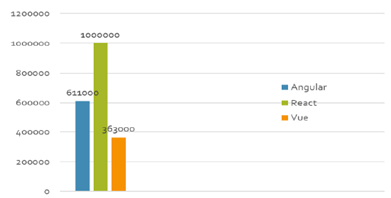
\includegraphics[width=0.6\textwidth]{image.png}
% \captionof{figure}{Number of GitHub repositories by frameworks~\cite{cincovic2020comparison}}
% \label{fig:github_repos}

\begin{figure}[h!]
    \centering
    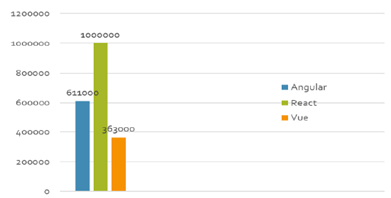
\includegraphics[width=0.6\textwidth]{image.png}
    \caption{Number of GitHub repositories by frameworks~\cite{cincovic2020comparison}}
    \label{fig:github_repos}
\end{figure}
    
% \begin{figure}[h]
% \centering
% 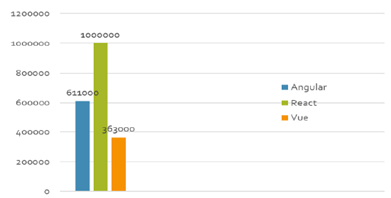
\includegraphics[width=0.6\textwidth]{image.png}
% \caption{Number of GitHub repositories by frameworks.}
% \label{fig
% }
% \end{figure}
% Active and engaged community support is crucial for framework development and bug fixing. Referring to the study by Jelica Cincović and Marija Punt titled "Comparison: Angular vs. React vs. Vue," which examined community support through GitHub repository comparisons, Figure  illustrates the following:

% \begin{figure}[h]
%     \centering
%     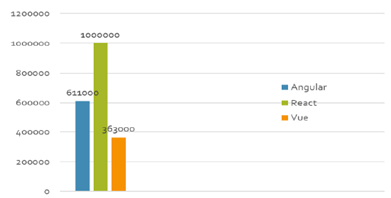
\includegraphics[width=0.6\textwidth]{image.png}
%     \caption{Number of GitHub repositories by frameworks}
%     \label{fig:github_repos}
% \end{figure}

% The graph indicates that React enjoys the largest community support, followed by Angular in second place and Vue in third~\cite{cincovic2020comparison}.
\newpage
\section{JavaScript for Complex Web Applications}

JavaScript is well-suited for complex web applications due to its versatility and the powerful features of modern JavaScript frameworks. These frameworks provide a structured environment for development, making it easier to manage large codebases and maintain code quality.

\textbf{Alternatives to JavaScript:}
\begin{itemize}
    \item \textbf{TypeScript:} A superset of JavaScript that adds static types, making it easier to catch errors early.
    \item \textbf{Dart:} Developed by Google, Dart is used in conjunction with the Flutter framework for building web and mobile apps.
    \item \textbf{Elm:} A functional language that compiles to JavaScript, focused on simplicity and quality tooling~\cite{mdn-js-guide}.
\end{itemize}

\section{Relevant JavaScript Web Application Frameworks}

Several JavaScript Web Application Frameworks are popular for developing web applications, each with its unique features and strengths. This section provides a brief overview of two of the most relevant frameworks, Vue.js and Angular, and explains why they are examined in detail.

\subsection{Angular}

Angular is a platform and framework for building single-page client applications using HTML and TypeScript. Developed by Google, Angular provides a comprehensive solution for complex and large-scale applications~\cite{angular-io}.

\textbf{Key Features:}
\begin{itemize}[label=\textbullet]
    \item \textbf{Two-way data binding:} Angular facilitates automatic synchronization of data between model and view components.
    \item \textbf{Dependency Injection:} Angular's DI system promotes modular development and testing by injecting dependencies into components.
    \item \textbf{Comprehensive CLI (Command-Line Interface):} Angular CLI offers powerful tools for project scaffolding, testing, and deployment.
    \item \textbf{TypeScript support:} Angular is built with TypeScript, providing type safety, enhanced tooling, and improved developer productivity.
\end{itemize}

\subsection{Vue}

Vue is a progressive JavaScript framework designed for building user interfaces. It is characterized by its incremental adoptability, allowing developers to integrate it gradually into existing projects without the need to fully commit to the entire framework upfront. This modular approach makes Vue suitable for both small-scale projects and large-scale applications, offering flexibility in usage based on project requirements~\cite{vuejs2024}.

\textbf{Key Features:}
\begin{itemize}[label=\textbullet]
    \item \textbf{Reactive data binding:} Vue's reactive system ensures efficient updates to the DOM based on changes in data.
    \item \textbf{Component-based architecture:} Vue promotes building UIs into modular, reusable components for easier maintenance and scalability.
    \item \textbf{Virtual DOM:} Vue uses a virtual DOM for efficient rendering and updating of the actual DOM elements.
    \item \textbf{Flexibility and integration:} Vue seamlessly integrates with existing projects and external libraries, offering flexibility in development approaches.
\end{itemize}

\section {Comparison Criteria - M}

When evaluating web development frameworks, metrics play a crucial role as they enable an objective analysis of performance and efficiency. By comparing load times, responsiveness, and resource utilization, frameworks like Angular and Vue can be assessed in various scenarios to determine their performance.

\subsection{Performance}
Angular provides robust performance and scalability for complex applications. In contrast, Vue stands out for its fast loading times and low overhead, making it particularly attractive for smaller projects~\cite{verma2022comparison}.

\subsection{Developer-friendliness}
Angular offers a robust structure and comprehensive features, which come with a steeper learning curve but are supported by extensive documentation and a strong community. Vue, on the other hand, is characterized by its easy integration and intuitive syntax, facilitating quicker onboarding and flexibility for smaller projects~\cite{angular, vue}.

\subsection{Community Support}
Active and engaged community support is crucial for framework development and bug fixing. Referring to the study by Jelica Cincović and Marija Punt titled "Comparison: Angular vs. React vs. Vue," which examined community support through GitHub repository comparisons, Figure  illustrates the following:

\begin{figure}[h]
    \centering
    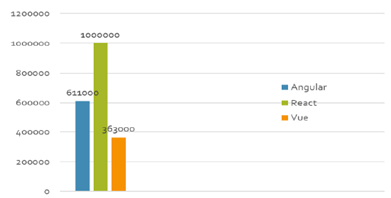
\includegraphics[width=0.6\textwidth]{image.png}
    \caption{Number of GitHub repositories by frameworks}
    \label{fig:github_repos}
\end{figure}

The graph indicates that React enjoys the largest community support, followed by Angular in second place and Vue in third~\cite{cincovic2020comparison}.

%\section{Brief Description of Angular.js}

%AngularJS, developed by Google, is a JavaScript framework for web development that emphasizes structure and quality. It was introduced in 2010 and was the first framework suitable for large enterprise applications, emphasizing clear architecture, high testability, and isolated components. Techniques like Dependency Injection enable efficient and maintainable software development based on JavaScript.

%Angular, introduced in 2016 as a successor to AngularJS, is a complete rewrite and uses TypeScript as its foundation. This allows for better scalability and performance. Angular offers an extensive development environment with features such as two-way data binding, a powerful Command Line Interface (CLI), and a well-defined architecture. It has evolved from a pure framework to a comprehensive platform for developing web applications \cite{angular}.

%\section{Brief Description of Vue.js}

%Vue.js, pronounced /vju:/, like "view", is a JavaScript framework for designing user interfaces. It was developed by Evan You in 2014 and has quickly become one of the most popular frameworks. Vue.js is based on standard HTML, CSS, and JavaScript and offers a declarative, component-based programming model. This model allows for efficient development of user interfaces of any complexity. Key features of Vue.js include the virtual DOM, reactive data binding, and easy integration with other projects and libraries.

%Vue.js is flexible and lightweight, suitable for both small projects and large applications. It allows developers to incrementally adopt it into existing projects and add additional features as needed \cite{vuejs}.

%\section{Differences Between Angular.js and Vue.js}

%Angular and Vue.js are both JavaScript frameworks that can be used to develop modern web applications. A key difference is that Angular uses an MVC (Model-View-Controller) architecture, while Vue.js is a more progressive framework.

%Angular provides a robust and well-established development environment with features such as efficient two-way data binding, a comprehensive CLI, and a well-defined architecture. It is particularly suitable for large and complex applications due to its strict structure and extensive tools.

%On the other hand, Vue.js is more flexible and lightweight. It uses a virtual DOM, which improves performance, and offers simple ways for CSS transitions and property computation. Vue.js is easier to learn and integrate, making it a good choice for smaller projects or projects that require rapid development.

%Both frameworks have their advantages and disadvantages, and the choice between them depends on the specific requirements and preferences of a project. While Angular offers a comprehensive solution for complex applications, Vue.js excels in simplicity and flexibility \cite{kinsta}.

\newpage

\section{Vue vs. Angular: A Detailed Comparison}

In this section, Vue and Angular will be compoared based on several parameters to provide a clear understanding of their respective strengths and weaknesses.

\subsection{Performance}

\textbf{Vue:}
\begin{itemize}
    \item Uses a virtual DOM for efficient updates
    \item Generally faster in rendering due to its lightweight nature
\end{itemize}

\textbf{Angular:}
\begin{itemize}
    \item Real DOM, which can be slower in certain scenarios
    \item Optimized for performance with techniques like ahead-of-time (AOT) compilation
\end{itemize}

\textbf{Comparison:}
\begin{itemize}
    \item Vue.js often has better performance for simple to moderately complex applications.
    \item Angular provides robust performance optimizations suitable for enterprise-level applications.
\end{itemize}

\subsection{Developer-Friendliness}

\textbf{Vue:}
\begin{itemize}
    \item Easy to learn and integrate
    \item Simple syntax and flexible structure
    \item Comprehensive documentation
\end{itemize}

\textbf{Angular:}
\begin{itemize}
    \item Steeper learning curve due to its complexity
    \item Requires understanding of TypeScript
    \item Extensive documentation and resources
\end{itemize}

\textbf{Comparison:}
\begin{itemize}
    \item Vue.js is generally more accessible for beginners.
    \item Angular is more suitable for developers with experience in TypeScript and complex frameworks.
\end{itemize}

\subsection{Community Support}

\textbf{Vue:}
\begin{itemize}
    \item Growing community with increasing adoption
    \item Numerous plugins and integrations
    \item Active development and support
\end{itemize}

\textbf{Angular:}
\begin{itemize}
    \item Large and established community
    \item Extensive resources and third-party libraries
    \item Backed by Google, ensuring long-term support
\end{itemize}

\textbf{Comparison:}
\begin{itemize}
    \item Angular has a larger and more established community.
    \item Vue.js is rapidly growing and has a supportive community.
\end{itemize}

\subsection{Ecosystem}

\textbf{Vue:}
\begin{itemize}
    \item Flexible and integrates well with other libraries
    \item Vue CLI for project scaffolding
    \item Vue Router and Vuex for state management
\end{itemize}

\textbf{Angular:}
\begin{itemize}
    \item Comprehensive suite of built-in tools
    \item Angular CLI for efficient development
    \item Angular Material for UI components
\end{itemize}

\textbf{Comparison:}
\begin{itemize}
    \item Vue.js offers flexibility in choosing tools and libraries.
    \item Angular provides a more integrated and consistent development experience.
\end{itemize}

\section{Conclusion}

Choosing the right framework depends on the specific needs of a project. Vue.js offers simplicity and flexibility, making it ideal for smaller projects and quick integration. Angular provides a comprehensive solution suitable for large-scale applications with its robust features and strong support from Google. Understanding the strengths and weaknesses of each framework can help developers make informed decisions to best meet their project requirements.
\chapter{Case Study - C}
\label{cha:CaseStudy}

%\section{Case Study}

%In this academic paper, a detailed case study of "ProTrack," an innovative web application engineered for tracking, sharing, managing, and collaboratively editing project work is presented. ProTrack is an invaluable resource for project management and providing tools that enhance administrative efficiency.

%ProTrack has been developed in two separate versions, one using Angular.js and the other with Vue.js. This dual-framework approach allows for a comprehensive comparison, providing clear insights into the unique benefits and potential limitations that each framework offers when applied to the same functional parameters.

%The case study section delves into several critical areas of ProTrack:
%\begin{itemize}
%    \item \textbf{Functionality}: The paper thoroughly explores ProTrack's essential features, including project tracking, document sharing, task management, and collaborative capabilities. It examines how each framework supports these features and assesses their impact on the user experience.
%    \item \textbf{Development Experience}: The section offers insights from the development process with Angular.js and Vue.js, focusing on tooling support and the ease of integration with other technologies.
%    \item \textbf{Performance Metrics}: Empirical data regarding performance metrics such as load times, runtime efficiency, and resource utilization for each framework are presented. This quantitative analysis enhances the qualitative evaluations provided throughout the case study.
%\end{itemize}

%Through this examination, the case study section aims to provide a detailed assessment of both frameworks as applied to a real-world application, thereby offering essential insights that assist developers and researchers in selecting between Angular.js and Vue.js for similar projects.

%\newpage

%\subsection*{Case Study 1: Angular.js Application}

%\begin{itemize}
%    \item \textbf{Functionality}:
%    \item \textbf{Development Experience}:
%    \item \textbf{Performance Metrics}:
%\end{itemize}

%\subsection*{Case Study 2: Vue.js Application}

%\begin{itemize}
%    \item \textbf{Functionality}:
%    \item \textbf{Development Experience}:
%    \item \textbf{Performance Metrics}:
%\end{itemize}

\section{Introduction to the Case Study}
\section{Application Description}
\section{Technical Implementation}
\section{Performance and efficiency}
\section{Challenges and Solutions}
\section{Comparison and analysis}
\section{Conclusion from the Case Study}
\chapter{Results - S}%
%- Ergebnisse Vergleichskriterien
%     -Leistung
%           - Benchmark-Tests und reale Beispiele, Vor- und Nachteile in verschiedenen Anwendungskriterien
%     -Community-Support und Ökosystem
%           - Anzahl und Aktivität der Community-Mitglieder
%           - Verfügbarkeit und Qualität von Bibliotheken und Tools
%

\section{Performance}
%unterschiede aufzeigen
\section{Developer-friendliness}
%unterschiede aufzeigen
\section{Community support}
%nochmal die unterschiede aufzählen aber nicht als pro con
\section{Ecosystem}
%nochmal die unterschiede aufzählen aber nicht als pro con
\chapter{Conclusion and recommendations - M}%
% - Fazit und Empfehlungen
%       - Zusammenfassung der Ergebnisse
%       - Empfehlungen für die Auswahl des geeigneten Frameworks
%       - Zukungsaussichten -> wie könnten sich die Frameworks weit‚erentwickeln

\section{Conclusion}


\section{Recommendations}
%wann würde sich welche Technologie empfehlen


\chapter[Case study]{Handling References to Literature and Other Sources}
\label{cha:Literature}


% \paragraph{Note:} The title of this chapter is intentionally lengthy, so it no
% longer fits in the page header. For this case, a shortened text for the header
% and the table of contents can be specified by providing an
% optional argument \verb![..]! to the \verb!\chapter! statement:
% %
% \begin{LaTeXCode}[numbers=none]
% \chapter[References to Literature]{Adding References to Literature and Other ...}
% \end{LaTeXCode}


% \section{General Remarks}

% The correct use of references is essential when writing scientific documents. Various guidelines are available for
% the design of references, determined among other things by the respective 
% subject area or guidelines from publishers and universities. 
% This template provides a scheme that is common in engineering and scientific
% disciplines.%
% \footnote{Adaptation to other specifications is relatively easy.}
% Technically, this part is based on the program \texttt{biber}%
% \footnote{\url{https://ctan.org/pkg/biber}}
% in combination with the \latex\ package \texttt{biblatex} \cite{Kime2023}.

% Reference management consists of two elements: \emph{citations} in the text
% refer to entries in the \emph{bibliography} (or multiple bibliographies). The
% bibliography is a compilation of all references, typically placed at the end of
% the document. Each citation must have an associated, unique entry in the
% bibliography; each item in the bibliography must likewise be referenced in the
% text.


% \section{Citations}

% Citations can be specified in several ways. Scenarios range from citing a single
% reference to references with additional information, such as a page number, to
% citing several different references simultaneously.

% \subsection{The \texttt{\textbackslash cite} Command}

% To create an entry in the bibliography and refer to it in the text, \latex\
% provides a central command. For citations in the running text, use the
% statement
% %
% \begin{itemize}
% \item[] \verb!\cite{!\textit{keys}\verb!}! \quad or \quad
% 				\verb!\cite[!\textit{text}\verb!]{!\textit{keys}\verb!}!.
% \end{itemize}
% %
% Here \textit{keys} is a comma-separated list of one or more citation keys to
% identify the corresponding entries in the bibliography, and \textit{text} can
% specify a supplementary text to the current citation, such as chapter or page
% references for books. Below are some examples:
% %
% \begin{itemize}
%     \item For further details, see \cite{Kopka2003}.
% \begin{LaTeXCode}[numbers=none]
% For further details, see \cite{Kopka2003}.
% \end{LaTeXCode}
% %
%     \item For further details, see \cite[Ch.~3]{Kopka2003}.
% \begin{LaTeXCode}[numbers=none]
% For further details, see \cite[Ch.~3]{Kopka2003}.
% \end{LaTeXCode}
% %
%     \item The data in \cite[pp.~274--277]{BurgeBurger1999} appear to be outdated.
% \begin{LaTeXCode}[numbers=none]
% The data in \cite[pp.~274--277]{BurgeBurger1999} appear to be  outdated.
% \end{LaTeXCode}
% %
%     \item Also important are \cite{Patashnik1988,Feder2006,Duden1997}.
% \begin{LaTeXCode}[numbers=none]
% Also important are \cite{Patashnik1988,Feder2006,Duden1997}.
% \end{LaTeXCode}
% \end{itemize}
% %
% In the last example, several references are listed in a single
% \texttt{\textbackslash cite} command. Note that the entries are sorted
% automatically (numerically or alphabetically). Multiple consecutive
% \texttt{\textbackslash cite} commands should not be used for this.

% \subsection{Multiple References With Additional Texts}

% Attaching texts to several sources simultaneously, for example, to indicate the
% respective page numbers, is complex. For this purpose, the
% \texttt{hagenberg-thesis} package offers the additional command%
% \footnote{\texttt{\textbackslash mcite} is defined in \texttt{hgbbib.sty} and
% works similar to the \texttt{{\bs}cites} command of \texttt{biblatex}
% (see \url{http://mirrors.ctan.org/macros/latex/contrib/biblatex/doc/biblatex.pdf}).}
% %
% \begin{itemize}
% \item[]
% \verb!\mcite[!\textit{text1}\verb!]{!\textit{key1}\verb!}!%
%       \verb![!\textit{text2}\verb!]{!\textit{key2}\verb!}!\ldots%
% 			\verb![!\textit{textN}\verb!]{!\textit{keyN}\verb!}!,
% \end{itemize}
% %
% where, for each given citation, key (\textit{key}) an associated \textit{text} can
% also be specified, for example:
% %
% \begin{itemize}
%     \item Similar results can be found in 
%     \mcite[Ch.~2]{Loimayr2019}[Sec.~3.6]{Drake1948}[pp.~5--7]{Eberl1987}.
% \begin{LaTeXCode}[numbers=none]
% Similar results can be found in 
% \mcite[Ch.~2]{Loimayr2019}[Sec.~3.6]{Drake1948}[pp.~5--7]{Eberl1987}.
% \end{LaTeXCode}
% \end{itemize}
% %
% For better readability, the output---unlike the regular
% \texttt{\textbackslash cite}---includes a \emph{semicolon} (;) as a separator
% between the entries. However, sorting the entries (if desired) must be done
% manually; it is not done by the \texttt{\textbackslash mcite} command.


% \subsection{Suppressing Back References in the Bibliography}

% With the present setup, a list of the text pages on which the source was cited
% is automatically appended to each entry in the bibliography. In rare cases, it
% is helpful to suppress these back references for individual citations, by using
% %
% \begin{itemize}
%     \item[] \verb!{\backtrackerfalse\cite{...}}!
% \end{itemize}
% %
% This also works with \verb!\mcite! and other \verb!cite! commands; note that 
% the outer brackets are important here. For example, in item
% {\backtrackerfalse\parencite{Bezos2023}} of the bibliography 
% the current page (\the\value{page}) should \emph{not} be listed.

% \subsection{Common Mistakes}

% Several common mistakes tend to occur when working with references, especially
% for inexperienced authors. However, these can be easily avoided.

% \subsubsection{Placing References Outside Sentences}

% Citations should be placed \emph{within} or\emph{at the end} of a sentence (\ie, before the
% period), not \emph{outside}:
% %
% \begin{quote}
% 	\begin{tabular}{rl}
% 		\textrm{Wrong:}  & \ldots this is the end of the sentence.
% 		\cite{Oetiker2021} And here it continues \ldots \\
% 		\textrm{Correct:} & \ldots this is the end of the sentence
% 		\cite{Oetiker2021}. And here it continues \ldots
% 	\end{tabular}
% \end{quote}

% \subsubsection{References Without a Preceding Space}

% A citation is \emph{always} separated from the preceding word by a space, never
% appended directly to the word (unlike a footnote):
% %
% \begin{quote}
% 	\begin{tabular}{rl}
% 		\textrm{Wrong:}  & \ldots here goes the
% 		citation\cite{Oetiker2021} and it continues \ldots  \\
% 		\textrm{Correct:} & \ldots here goes the citation
% 		\cite{Oetiker2021} and it continues \ldots
% 	\end{tabular}
% \end{quote}

% \subsubsection{Literal Quotes}

% If an entire paragraph (or more) is quoted from a source, the associated reference
% should
% be placed in the preceding text and not \emph{within} the quote itself. As an
% example, the following passage from \cite{Daniel2018}:
% %
% \begin{quote}
% 	\begin{german}
% 		Typographisches Design ist ein Handwerk, das erlernt werden muss.
% 		Ungeübte Autoren machen dabei oft gravierende Fehler. Fälschlicherweise
% 		glauben viele Laien, dass Textdesign vor allem eine Frage der Ästhetik
% 		ist -- wenn das Schriftstück vom künstlerischen Standpunkt aus "schön"
% 		aussieht, dann ist es schon gut "designed". Da Schriftstücke jedoch
% 		gelesen und nicht in einem Museum aufgehängt werden, sind die leichtere
% 		Lesbarkeit und bessere Verständlichkeit wichtiger als das schöne
% 		Aussehen.
% 	\end{german}
% \end{quote}
% %
% For the quote itself, the \texttt{quote} environment should be used; it
% demarcates the quote from one's text by employing indentations on both sides and
% thus reduces the risk of ambiguities (where is the end of the quote?). The above
% example also switches to German (see Sec.\ \ref{sec:language-switching}):%
% \footnote{Note the German quotation marks inside the quote, which
% are set by the \texttt{smartquotes} option.}
% %
% \begin{itemize}
%     \item[] \verb!\begin{quote}\begin{german}! \emph{quoted text \ldots}
%     \verb!\end{german}\end{quote}!
% \end{itemize}
% %
% If desired, the quote can also be wrapped in quotation marks \emph{or}
% italicized, but not both!

% \subsubsection{Optional Extensions (Using Document Option
% \texttt{smartquotes})}

% The \texttt{csquotes} package%
% \footnote{\url{https://ctan.org/pkg/csquotes}, see also section
% \ref{sec:quotation-marks}.}
% (automatically loaded by the \texttt{smartquotes} option) defines several
% additional environments for quotes, \eg
% %
% \begin{itemize}
%     \item[] \verb!\begin{displayquote}! \ldots \verb!\end{displayquote}!
% \end{itemize}
% %
% (equivalent to \verb!\begin{quote}! \ldots \verb!\end{quote}!) and for foreign
% language quotes the environment
% %
% \begin{itemize}
%     \item[] \verb!\begin{foreigndisplayquote}{language}! \ldots
%     \verb!\end{foreigndisplayquote}!.
% \end{itemize}
% %
% This allows, for example, a German quote%
% \footnote{Currently, only the languages \texttt{german} and \texttt{english}
% are defined.}
% \emph{without} explicit language switching:
% %
% \begin{itemize}
%     \item[] \verb!\begin{foreigndisplayquote}{german}!\newline
%        \verb!   !\emph{quoted text \ldots}\newline
%     \verb!\end{foreigndisplayquote}!
% \end{itemize}

% \subsection{Dealing With Secondary Sources}

% In rare cases, it happens that one wants (or needs) to cite a source \textrm{A}
% that is not available (and thus cannot be read personally) but which is cited in
% \emph{another} available source \textrm{B}. In this case, \textrm{A} is called
% the \emph{original} or \emph{primary source}, and \textrm{B} is called the
% \emph{secondary source}. In such a scenario the following basic rules should be
% observed:
% %
% \begin{itemize}
%     \item Secondary sources should be \emph{avoided} whenever
%     possible.
%     \item In order to quote a source in the usual form, one must always have
%     \emph{personally accessed} (read) it!
%     \item Only if one can absolutely \emph{not} get hold of the primary source, a
%     reference via a secondary source is permissible. In this case, primary and
%     secondary sources should be \emph{cited together}, as shown in the example
%     below.
%     \item \emph{Important}: Only the available source (\textrm{B}) and not
%     the original work is included in the bibliography!
% \end{itemize}
% %
% \paragraph{Example:} Suppose one would like to quote a passage from the famous
% book (\textrm{A}) \emph{Dialogo} by Galileo Galilei (which is difficult to obtain),
% referenced in a more recent work from 1969 (\textrm{A}). One could accomplish this,
% \eg, with the following footnote (all page numbers are fictional).%
% \footnote{Galileo Galilei, \emph{Dialogo sopra i due massimi sistemi del
% mondo tolemaico e copernicano}, p.~314 (1632). Quoted from 
% \cite[p.~59]{Hemleben1969}.}
% Only the secondary source \cite{Hemleben1969} is included in the actual bibliography.


% \section{Bibliography}

% There are several options for creating the bibliography in \latex. The
% traditional method is to use \texttt{BibTeX} \cite{Patashnik1988}. Another (more
% modern) approach uses \texttt{biber}%
% \footnote{\url{http://mirrors.ctan.org/biblio/biber/documentation/biber.pdf}}
% and \texttt{biblatex}, as described below.


% \subsection{Bibliographic Data in BibTeX and BibLaTex}
% \label{sec:bibtex}

% BibTeX is a stand-alone program that generates a bibliography suitable for
% \latex from a "bibliographic database" (one or more text files with a given
% structure). Literature on using BibTeX can be found online, \eg,
% \cite{Feder2006, Patashnik1988}.

% BibTeX files can, of course, be created manually with a text editor. For many
% references, complete BibTeX entries are already available online. However, one
% should be careful because these entries are (even when provided by large
% institutions and publishers) \emph{often wrong or syntactically incorrect}!
% Therefore, one should not adopt them unchecked and especially scrutinize the
% final results. Furthermore, there are specialized applications for maintaining
% BibTeX bibliographies, such as \emph{JabRef}.%
% \footnote{\url{https://www.jabref.org/}}

% \subsubsection{Using \texttt{biblatex} and \texttt{biber}}

% This document uses \texttt{biblatex} (version 1.4 or higher) in conjunction with
% the software \texttt{biber}, which addresses many shortcomings of the
% traditional BibTeX workflow and significantly extends its capabilities.%
% \footnote{In fact, \texttt{biblatex} is the first radical (and long-needed)
% overhaul of the outdated BibTeX workflow and has already replaced the latter in
% many documents.}
% It adds many new entry types, which are indispensable, especially for
% referencing modern multimedia sources. However, this means that the
% bibliographic data used in \texttt{biblatex} are no longer fully backward
% compatible with BibTeX. It is, therefore, usually necessary to manually revise
% existing BibTeX data or data taken from online sources (see
% Section~\ref{sec:tips-on-biblatex}).

% In our setup, the interface to \texttt{biblatex} is contained in the style
% file \nolinkurl{hgbbib.sty}. The typical usage in the main \latex file is as
% follows:
% %
% \begin{LaTeXCode}[numbers=left]
% \documentclass[master,english,smartquotes]{hgbthesis}
%    ...
% \bibliography{references} /+\label{tex:references1}+/
%    ...
% \begin{document}
%    ...
% \MakeBibliography /+\label{tex:references2}+/
%    ...
% \end{document}
% \end{LaTeXCode}
% %
% In the "preamble",
% \verb!\bibliography{references}!%
% \footnote{The \texttt{{\bs}bibliography} command is actually a relic from BibTeX
% and is replaced in \texttt{biblatex} by the \texttt{{\bs}addbibresource}
% statement. Both statements are equivalent, but often only
% \texttt{{\bs}bibliography} makes the associated \texttt{.bib} file visible in
% the file structure of the editor environment.}
% (line \ref{tex:references1}) refers to a BibLaTeX file \nolinkurl{references.bib},
% which holdss all references.
% If multiple BibLaTeX files are used, they can be specified in the same form.

% The \verb!\MakeBibliography! statement near the end of the document
% (line~\ref{tex:references2}) is responsible for the output of the bibliography,
% here with the title "References". Two variants are possible:
% %
% \begin{description}
%     \item[\texttt{{\bs}MakeBibliography}] ~ \newline
%     Creates a bibliography divided into several \emph{categories} (see
%     Section~\ref{sec:reference-categories}). This variant is used in the present
%     document.
% %
%     \item[\texttt{{\bs}MakeBibliography[nosplit]}] ~ \newline
%     Generates a traditional \emph{one-piece} bibliography.
% \end{description}

% \subsection{Reference Categories}
% \label{sec:reference-categories}

% The \texttt{hagenberg-thesis} package provides the following categories for split
% bibliographies (see Table~\ref{tab:references-and-entry-types}):%.
% \footnote{These categories are defined in the file \nolinkurl{hgbbib.sty}. Any
% changes and the definition of additional categories are pretty straightforward
% if required.}
% %
% \begin{itemize}
%     \item[] \textsf{literature} -- for classic publications that are available
%     in print or online;
%     \item[] \textsf{avmedia} -- for movies, audio-visual media (on DVD,
%     streaming, \etc);
%     \item[] \textsf{software} -- for software, APIs, computer games;
%     \item[] \textsf{online} -- for artifacts that are \emph{only} available
%     online.
% \end{itemize}
% %
% Each reference is automatically assigned to one of these categories based on the
% specified BibLaTeX entry type (\texttt{@\emph{type}}) (see
% Table~\ref{tab:reference-categories}). Only the most essential entry types are
% listed here, but they should cover most cases in practice and are explained
% below by examples. All entries that are not explicitly specified are assigned to
% the category \textsf{literature}.


% %%------------------------------------------------------

% \begin{table}[htbp]
% \caption{Defined reference categories and recommended BibLaTeX entry types.}
% \label{tab:references-and-entry-types}
% \centering
% \begin{tabular}{@{}llc@{}}
% 	\toprule
% 	\emph{Literature} (\textsf{literature}) & Type & Page\\
% 	\midrule
% 	Book (textbook, monograph) & \texttt{@book} & \pageref{sec:@book}\\
% 	Collection (editor and multiple authors) & \texttt{@incollection} & \pageref{sec:@incollection} \\
% 	Conference proceedings & \texttt{@inproceedings} & \pageref{sec:@inproceedings}\\
% 	Article in a journal or magazine & \texttt{@article} & \pageref{sec:@article}\\
% 	Thesis (bachelor, master, diploma), dissertation & \texttt{@thesis} & \pageref{sec:@thesis}\\
% 	Technical report, lab report & \texttt{@report} & \pageref{sec:@report}\\
% 	Manual, product description & \texttt{@manual} & \pageref{sec:@manual}\\
% 	Norm, standard & \texttt{@standard} & \pageref{sec:@standard}\\
% 	Laws, bills, regulations, \etc & \texttt{@legislation} & \pageref{sec:@legislation}\\
% 	Compositions, sheet music & \texttt{@book}, \texttt{@incollection} & \pageref{sec:sheet-music}\\
% 	Pre-publications (\eg conference submissions) & \texttt{@unpublished} & \pageref{sec:@unpublished}\\
% 	\addlinespace
% %
% 	\midrule
% 	\emph{Audiovisual media} (\textsf{avmedia}) & & \\
% 	\midrule
% 	Audio (CD) & \texttt{@audio} & \pageref{sec:@audio}\\
% 	Image, photo, graphic & \texttt{@image} & \pageref{sec:@image}\\
% 	Video (on DVD, Blu-ray disk, online) & \texttt{@video} & \pageref{sec:@video}\\
% 	Movie (cinema) & \texttt{@movie} & \pageref{sec:@movie}\\
% 	\addlinespace
% %
% 	\midrule
% 	\emph{Software} (\textsf{software}) & & \\
% 	\midrule
% 	Software product or project & \texttt{@software} & \pageref{sec:@software}\\
% 	Computer game & \texttt{@software} & \pageref{sec:@software}\\
% 	\addlinespace
% %
% 	\midrule
% 	\emph{Online sources} (\textsf{online}) & & \\
% 	\midrule
% 	Website, wiki entry, blog, \etc & \texttt{@online} & \pageref{sec:@online-www} \\
% 	\bottomrule
% \end{tabular}
% \end{table}

% \begin{table}
% \caption{Reference categories and associated BibLaTeX entry types. In the case
% of a split bibliography, the entries of each category are combined in a
% common section. Items marked in gray are synonyms for the respective
% types above them.}
% \label{tab:reference-categories}
% \centering
% \definecolor{midgray}{gray}{0.5}
% \setlength{\tabcolsep}{4mm}
% \begin{tabular}{@{}llll@{}}
% 	\toprule
% 	\textsf{literature} & \textsf{avmedia} & \textsf{software} & \textsf{online} \\
% 	\midrule
% 	\texttt{@book} & \texttt{@audio} & \texttt{@software} & \texttt{@online} \\
% 	\texttt{@incollection} & \texttt{\color{midgray}@music} & & \texttt{\color{midgray}@electronic} \\
% 	\texttt{@inproceedings} & \texttt{@video} & & \texttt{\color{midgray}@www} \\
% 	\texttt{@article} & \texttt{@movie} & & \\
% 	\texttt{@thesis} & \texttt{@software} & & \\
% 	\texttt{@report} & & & \\
% 	\texttt{@manual} & & & \\
% 	\texttt{@standard} & & & \\
% 	\texttt{@legislation} & & & \\
% 	\texttt{@misc} & & &  \\
% 	\texttt{@unpublished} &  & & \\
% 	\ldots & & & \\
% 	\bottomrule
% \end{tabular}
% \end{table}

% %% ----------------------------------------------------

% \subsection{Printed Sources (\textsf{literature})}
% \label{sec:category-literature}

% This category includes all works published in printed form, for example, in
% books, conference proceedings, journal articles, theses, etc. In the following
% examples, the BibLaTeX entry in the file \nolinkurl{references.bib} is given,
% followed by the corresponding result in the bibliography.

% \subsubsection{\texttt{\bfseries @book}}
% \label{sec:@book}

% A single-volume book (monograph) written in its entirety by one or more authors
% and (typically) published by one publisher.
% % 
% \begin{itemize}
% \item[]
% \begin{GenericCode}[numbers=none]
% @book{BurgerBurge2022,
% 	author={Burger, Wilhelm and Burge, Mark James},
% 	title={Digital Image Processing},
% 	subtitle={An Algorithmic Introduction},
% 	publisher={Springer},
% 	location={Cham},
% 	edition={3},
% 	date={2022},
% 	doi={10.1007/978-3-031-05744-1},
% 	langid={english}
% }
% \end{GenericCode}
% \item[\cite{BurgerBurge2022}] \fullcite{BurgerBurge2022}
% \end{itemize}
% %
% Note: The entry field \texttt{edition} is usually only specified if there
% is \emph{more} than one, especially \emph{not for the first
% edition} if this is the only one! ISBNs can be safely omitted.


% %%------------------------------------------------------

% \subsubsection{\texttt{\bfseries @incollection}}
% \label{sec:@incollection}

% A self-contained and titled contribution by one or more authors to a book or
% collection. \texttt{title} is the title of the contribution, \texttt{booktitle}
% the title of the collection, and \texttt{editor} the name of the editor.
% %
% \begin{itemize}
% \item[]
% \begin{GenericCode}[numbers=none]
% @incollection{BurgeBurger1999,
%   author={Burge, Mark and Burger, Wilhelm},
%   title={Ear Biometrics},
%   booktitle={Biometrics},
%   booksubtitle={Personal Identification in Networked Society},
%   publisher={Kluwer Academic Publishers},
%   date={1999},
%   location={Boston},
%   editor={Jain, Anil K. and Bolle, Ruud and Pankanti, Sharath},
%   chapter={13},
%   pages={273-285},
%   doi={10.1007/0-306-47044-6_13},
%   langid={english}
% }
% \end{GenericCode}
% \item[\cite{BurgeBurger1999}] \fullcite{BurgeBurger1999}
% \end{itemize}


% %%------------------------------------------------------

% \subsubsection{\texttt{\bfseries @inproceedings}}
% \label{sec:@inproceedings}

% Conference paper, individual contribution in conference proceedings. Distinguish
% between the fields \texttt{venue} to indicate the place of the conference and
% \texttt{location} for the location of the publisher.
% %
% \begin{itemize}
% \item[]
% \begin{GenericCode}[numbers=none]
% @inproceedings{Burger1987,
%   author={Burger, Wilhelm and Bhanu, Bir},
%   title={Qualitative Motion Understanding},
%   booktitle={Proceedings of the Tenth International Joint Conference on Artificial Intelligence},
%   date={1987-08},
%   editor={McDermott, John P.},
%   eventdate={1987-08-23/1987-08-28},
%   venue={Milano},
%   publisher={Morgan Kaufmann Publishers},
%   location={San Francisco},
%   pages={819-821},
%   doi={10.1007/978-1-4615-3566-9},
%   langid={english}
% }
% \end{GenericCode}
% \item[\cite{Burger1987}] \fullcite{Burger1987}
% \end{itemize}

% %%------------------------------------------------------

% \subsubsection{\texttt{\bfseries @article}}
% \label{sec:@article}

% Article in a magazine, scientific journal, or daily newspaper. \texttt{volume}
% denotes the volume and \texttt{number} the number within that volume. The
% journal name (\texttt{journaltitle}) should be abbreviated only in justifiable
% cases to avoid misunderstandings.
% %
% \begin{itemize}
% \item[]
% \begin{GenericCode}[numbers=none]
% @article{Mermin1989,
%   author={Mermin, Nathaniel David},
%   title={What's Wrong with these Equations?},
%   journaltitle={Physics Today},
%   volume={42},
%   number={10},
%   date={1989},
%   pages={9-11},
%   doi={10.1063/1.2811173},
%   langid={english}
% }
% \end{GenericCode}
% \item[\cite{Mermin1989}] \fullcite{Mermin1989}
% \end{itemize}
% %
% Note: Specifying an issue for \emph{multiple} months (for example, in the
% case of a combined issue) is not possible in \texttt{biblatex} with the
% \texttt{month} field because it may only contain \emph{a single} number.
% However, the \texttt{number} field can be used for this purpose, \eg,
% \texttt{number=\{6-7\}} in \cite{Vardavoulia2001}.

% %%------------------------------------------------------

% \subsubsection{\texttt{\bfseries @thesis}}
% \label{sec:@thesis}

% This entry type can be used for any academic thesis. The exact type is specified via the
% \texttt{type} attribute. The values \texttt{phdthesis}, \texttt{mathesis}, and
% \texttt{bathesis} indicate doctoral, master's, and bachelor's theses,
% respectively, and correctly specify the type of thesis, depending on the
% document language and style. Alternatively, individual content can be stored in
% this field.

% \paragraph{Dissertation (Doctoral Thesis, PhD Thesis):}
% %
% \begin{itemize}
% \item[]
% \begin{GenericCode}[numbers=none]
% @thesis{Eberl1987,
%   author={Eberl, Gerhard},
%   title={Automatischer Landeanflug durch Rechnersehen},
%   type={phdthesis},
%   date={1987-08},
%   institution={Universität der Bundeswehr, Fakultät für Raum- und Luftfahrttechnik},
%   location={München},
%   langid={ngerman}
% }
% \end{GenericCode}
% \item[\cite{Eberl1987}] \fullcite{Eberl1987}
% \end{itemize}

% \paragraph{Diploma Thesis:} ~ \newline
% Equivalent to a dissertation (see above), but with
% \texttt{type=\obnh\{Diploma thesis\}}.

% %%------------------------------------------------------

% \paragraph{Master Thesis:} ~ \newline
% Equivalent to a dissertation (see above), but with \texttt{type=\{mathesis\}}.%

% %
% \begin{itemize}
% \item[]
% \begin{GenericCode}[numbers=none]
% @thesis{Loimayr2019,
%   author={Loimayr, Nora},
%   title={Utilization of GPU-Based Smoothed Particle Hydrodynamics for Immersive Audiovisal Experiences},
%   type={mathesis},
%   date={2019-11-26},
%   month={11},
%   institution={University of Applied Sciences Upper Austria, Interactive Media},
%   location={Hagenberg, Austria},
%   url={https://theses.fh-hagenberg.at/thesis/Loimayr19},
%   langid={english}
% }
% \end{GenericCode}
% \item[\cite{Loimayr2019}] \fullcite{Loimayr2019}
% \end{itemize}
% %
% The content of the \verb!url={..}! field will be automatically typeset as a URL
% without any additional markup (using the \verb!\url{..}! command).

% %%------------------------------------------------------

% \paragraph{Bachelor Thesis:} ~ \newline
% Bachelor theses are not usually considered "proper" publications, but it must
% still be possible to reference them if necessary, for example:
% %
% \begin{itemize}
% \item[]
% \begin{GenericCode}[numbers=none]
% @thesis{Bacher2004,
%   author={Bacher, Florian},
%   title={Interaktionsmöglichkeiten mit Bildschirmen und großflächigen Projektionen},
%   type={bathesis},
%   date={2004-06},
%   institution={University of Applied Sciences Upper Austria, Medientechnik und {-design}},
%   location={Hagenberg, Austria},
%   langid={ngerman}
% }
% \end{GenericCode}
% \item[\cite{Bacher2004}] \fullcite{Bacher2004}
% \end{itemize}

% %%------------------------------------------------------

% \subsubsection{\texttt{\bfseries @report}}
% \label{sec:@report}

% These are typically numbered reports (\emph{technical reports} or \emph{research
% reports}) from companies, university institutes, or research projects. They are
% distinguished by the \texttt{type} attribute, which can take the values
% \texttt{techreport} or \texttt{resreport}. Specifying the issuing organizational
% unit (company, institute, faculty, \etc) and address is essential. It also makes
% sense to provide a corresponding URL, if available.
% %
% \begin{itemize}
% \item[]
% \begin{GenericCode}[numbers=none]
% @report{Drake1948,
%   author={Drake, Hubert M. and McLaughlin, Milton D. and Goodman, Harold R.},
%   title={Results obtained during accelerated transonic tests of the {Bell} {XS-1} airplane in flights to a {MACH} number of 0.92},
%   type={techreport},
%   institution={NASA Dryden Flight Research Center},
%   date={1948-01},
%   location={Edwards, CA},
%   number={NACA-RM-L8A05A},
%   url={https://www.nasa.gov/centers/dryden/pdf/87528main_RM-L8A05A.pdf},
%   langid={english}
% }
% \end{GenericCode}
% \item[\cite{Drake1948}] \fullcite{Drake1948}
% \end{itemize}

% %%------------------------------------------------------

% \subsubsection{\texttt{\bfseries @manual}}
% \label{sec:@manual}

% This publication type is suitable for technical or other documentation, such as
% product descriptions, manuals, presentations, white papers, \etc The
% documentation does not need to exist in printed form.
% %
% \begin{itemize}
% \item[]
% \begin{GenericCode}[numbers=none]
% @manual{Mittelbach2023,
%   author={Mittelbach, Frank and Schöpf, Rainer and Downes, Michael and Jones, David M. and Carlisle, David},
%   title={The \texttt{amsmath} package},
%   date={2023-05-13},
%   version={2.17o},
%   url={http://mirrors.ctan.org/macros/latex/required/amsmath/amsmath.pdf},
%   langid={english}
% }
% \end{GenericCode}
% \item[\cite{Mittelbach2023}] \fullcite{Mittelbach2023}
% \end{itemize}
% %
% Often no author is named in such documents. Instead, the name of the
% \emph{company} or \emph{institution} is specified in the \texttt{author} field,
% but within \emph{additional parentheses} \texttt{\{..\}}, so that the
% argument is not misinterpreted as \emph{first name} + \emph{last name}.%.
% \footnote{Unlike BibTeX, \texttt{biblatex} does not accept the
% \texttt{organization} field as a replacement for \texttt{author} in
% \texttt{@manual} entries.}
% This trick is used in the following example (among others).

% %%------------------------------------------------------

% \subsubsection{\texttt{\bfseries @standard}}
% \label{sec:@standard}

% References to \emph{standards} are supported in \texttt{biblatex} through the
% type \texttt{@standard}. Here is a typical example:
% %
% \begin{itemize}
% \item[]
% \begin{GenericCode}[numbers=none]
% @standard{WHATWGHTMLLivingStandard,
%   author={{Web Hypertext Application Technology Working Group}},
%   shortauthor={WHATWG},
%   title={HTML},
%   titleaddon={Living Standard},
%   date={2023-11-06},
%   url={https://html.spec.whatwg.org/multipage/},
%   langid={english}
% }
% \end{GenericCode}
% \item[\cite{WHATWGHTMLLivingStandard}] \fullcite{WHATWGHTMLLivingStandard}
% \end{itemize}
% %

% %%------------------------------------------------------

% \subsubsection{\texttt{\bfseries @patent}}
% \label{sec:@patent}

% The special entry type \texttt{@patent} exists for patents, as the following
% example shows. \texttt{year} and \texttt{month} refer to the date of the patent
% grant; the specification of \texttt{holder} is optional:
% %
% \begin{itemize}
% \item[]
% \begin{GenericCode}[numbers=none]
% @patent{Pike2008,
%   author={Pike, Dion},
%   title={Master-slave communications system and method for a network element},
%   type={US Patent},
%   holder={Alcatel-Lucent SAS},
%   number={7,460,482},
%   date={2008-12-02},
%   url={https://patents.google.com/patent/US7460482},
%   langid={english}
% }
% \end{GenericCode}
% \item[\cite{Pike2008}] \fullcite{Pike2008}
% \end{itemize}
% %

% %%------------------------------------------------------

% \subsubsection{\texttt{\bfseries @legislation}}
% \label{sec:@legislation}

% Legal texts can be mapped in \texttt{biblatex} using the type
% \texttt{@legislation}. Since this is a non-standard type, the driver for
% \texttt{@misc} is used, so it is essential to specify details such as the type
% of publication with the \texttt{howpublished} field. The following example shows
% the application for a legal text (see also \cite{FhStG1993} and
% \cite{EuRichtlinie2000}).
% %
% \begin{itemize}
% \item[]
% \begin{GenericCode}[numbers=none]
% @legislation{OoeRaumordnungsgesetz1994,
%   title={Landesgesetz vom 6. Oktober 1993 über die Raumordnung im Land Oberösterreich},
%   titleaddon={Oö. Raumordnungsgesetz 1994 - Oö. ROG 1994},
%   howpublished={LGBl.Nr. 114/1993 zuletzt geändert durch LGBl.Nr. 111/2022},
%   date={1993-12-23},
%   url={https://www.ris.bka.gv.at/GeltendeFassung.wxe?Abfrage=LrOO&Gesetzesnummer=10000370},
%   langid={ngerman}
% }
% \end{GenericCode}
% \item[\cite{OoeRaumordnungsgesetz1994}] \fullcite{OoeRaumordnungsgesetz1994}
% \end{itemize}
% %

% %%------------------------------------------------------

% \subsubsection{\texttt{\bfseries @misc}}
% \label{sec:@misc}

% If the entry types for printed publications listed so far do not suffice, one
% should first look at the other types (not described in detail here) in the
% \texttt{biblatex} manual \cite{Kime2023}. For example, \texttt{@collection} for
% a complete collection (\ie, not just a single contribution).

% If none of them fit, then the \texttt{@misc} type can be used. It provides a
% \texttt{howpublished} text field where the type of publication can be specified
% individually. Likewise, the \texttt{type} field can be used to specify what kind
% of document is represented.

% %%------------------------------------------------------

% \subsubsection{Compositions and Sheet Music}
% \label{sec:sheet-music}

% For printed compositions (sheet music or musical scores), there is,
% unfortunately, no particular entry type in BibLaTeX. For a \emph{specific}
% edition, it is easiest to use the type \texttt{@book}, such as (see also
% \cite{HaydnCelloConcerto2,ShostakovichOp110})
% %
% \begin{itemize}
% \item[]
% \begin{GenericCode}[numbers=none]
% @book{BachBWV988,
%   author={Bach, Johann Sebastian},
%   title={Goldberg-Variationen für Streichquartett, BWV 988},
%   editor={Anka, Dana},
%   publisher={Musikverlag Hans Sikorski},
%   location={Hamburg},
%   date={2017},
%   langid={ngerman}
% }
% \end{GenericCode}
% \item[\cite{BachBWV988}] \fullcite{BachBWV988}
% \end{itemize}
% %
% For compositions that have been published in a collection, one can use---as for
% a scientific collection---the type \texttt{@incollection}:
% %
% \begin{itemize}
% \item[]
% \begin{GenericCode}[numbers=none]
% @incollection{GershwinSummertime,
%   author={Gershwin, George and Heyward, DuBose},
%   title={Summertime},
%   booktitle={The Greatest Songs of George Gershwin},
%   publisher={Chappel Music},
%   location={London},
%   pages={40-43},
%   date={1979},
%   langid={english}
% }
% \end{GenericCode}
% \item[\cite{GershwinSummertime}] \fullcite{GershwinSummertime}
% \end{itemize}

% \subsubsection{\texttt{\bfseries @unpublished}}
% \label{sec:@unpublished}

% It is becoming increasingly common for manuscripts to be published online by
% authors a long time before actual publication, for example, on platforms such as
% \textsf{arXiv.org}%
% \footnote{\url{https://arxiv.org/}}
% or \textsf{researchgate.net}.%
% \footnote{\url{https://www.researchgate.net/}}
% It should be noted that releasing something online does \emph{not formally
% count as a publication}, as these platforms are no publishers. Some of the
% works (uploaded by the authors) are \emph{never} officially published, \eg,
% unaccepted submissions to conferences. When citing this reference it is crucial
% to determine whether the paper was accepted and actually published:
% %
% \begin{itemize}
% \item[a)]
% \emph{The work was indeed published:} Here the corresponding original
% publication must be searched and used! The citation is done in conventional form
% (for example, with \texttt{@inproceedings} in case of a conference volume), but
% \emph{without} a reference to the online publication.
% \item[b)]
% \emph{The work was \emph{not} published:} If indeed no publication (or an
% associated \emph{technical report}, see above) can be found, the
% \texttt{@unpublished} tag can be helpful:
% \item %
% \begin{GenericCode}[numbers=none]
% @unpublished{Dai2016,
%   author={Dai, Jifeng and Li,Yi and He, Kaiming and Sun, Jian},
%   title={{R-FCN:} Object Detection via Region-Based Fully Convolutional Networks},
%   date={2016},
%   pubstate={prepublished},
%   doi={10.48550/arXiv.1605.06409},
%   langid={english}
% }
% \end{GenericCode}
% \begin{itemize}
% \item[\cite{Dai2016}] \fullcite{Dai2016}
% \end{itemize}
% %
% \end{itemize}
% %
% In the latter case, the specification of the link (via \texttt{doi} or alternatively
% \texttt{url}) is essential. Details on the \texttt{pubstate} field
% (\texttt{prepublished}) can be found in the \texttt{biblatex} documentation
% \cite[Sec.\ 4.9.2.11]{Kime2023}. Otherwise (if unknown or not published),
% %
% \begin{itemize}
% \item[]\texttt{note=\{unpublished\}} \quad or
%    \quad \texttt{note=\{unververöffentlicht\}}
% \end{itemize}
% %
% can be used instead of \texttt{pubstate}.


% \subsection{Movies and Audio-Visual Media (\textsf{avmedia})}
% \label{sec:category-avmedia}

% This category covers audio-visual productions such as movies, sound recordings,
% CDs, DVDs, and VHS tapes, thus meaning works published in physical (but not
% printed) form. It does not include audio-visual creations (sound recordings,
% images, videos) that are exclusively available online---these should be
% referenced with the entry type \texttt{@online} (see
% Table~\ref{tab:reference-categories} and Section~\ref{sec:category-online}).

% The \texttt{@audio}, \texttt{@video}, and \texttt{@movie} types described below
% are \emph{not} BibTeX standard types. However, they are represented in
% \texttt{biblatex} (implicitly replaced by \texttt{@misc}) and are recommended
% here to allow the automatic assignment of items in the bibliography.

% \subsubsection{\texttt{\bfseries @audio}}
% \label{sec:@audio}
% Here is an example of the specification of an audio CD:
% %
% \begin{itemize}
% \item[]
% \begin{GenericCode}[numbers=none]
% @audio{Zappa1995,
%   author={Zappa, Frank},
%   title={Freak Out!},
%   type={audiocd},
%   date={1995-05},
%   organization={Rykodisc, New York},
%   langid={english}
% }
% \end{GenericCode}
% \item[\cite{Zappa1995}] \fullcite{Zappa1995}
% \end{itemize}
% %
% Instead of \verb!type={audiocd}! one could also use \verb!howpublished={Audio CD}!.

% \subsubsection{\texttt{\bfseries @image}}
% \label{sec:@image}

% The following example shows the reference to a digitally available photo, which
% is also used in Figure~\ref{fig:CocaCola}:
% %
% \begin{itemize}
% \item[]
% \begin{GenericCode}[numbers=none]
% @image{CocaCola1940,
%   author={Wolcott, Marion Post},
%   title={Natchez, Miss.},
%   note={Library of Congress Prints and Photographs Division Washington, Farm Security Administration/Office of War Information Color Photographs},
%   date={1940-08},
%   url={https://www.loc.gov/pictures/item/2017877479/},
%   langid={english}
% }
% \end{GenericCode}
% \item[\cite{CocaCola1940}] \fullcite{CocaCola1940}
% \end{itemize}

% \subsubsection{\texttt{\bfseries @video}}
% \label{sec:@video}

% The example below shows a link to a YouTube video:
% %
% \begin{itemize}
% \item[]
% \begin{GenericCode}[numbers=none]
% @video{HistoryOfComputers2008,
%   title={History of Computers},
%   date={2008-09-24},
%   url={https://www.youtube.com/watch?v=LvKxJ3bQRKE},
%   langid={english}
% }
% \end{GenericCode}
% \item[\cite{HistoryOfComputers2008}] \fullcite{HistoryOfComputers2008}
% \end{itemize}

% \noindent
% Here is an example of referencing a DVD edition:
% %
% \begin{itemize}
% \item[]
% \begin{GenericCode}[numbers=none]
% @video{Futurama1999,
%   author={Groening, Matt},
%   title={Futurama},
%   titleaddon={Season 1 Collection},
%   howpublished={DVD},
%   date={2002-02},
%   organization={Twentieth Century Fox Home Entertainment},
%   langid={english}
% }
% \end{GenericCode}
% \item[\cite{Futurama1999}] \fullcite{Futurama1999}
% \end{itemize}
% %
% In this case, the specified date is the \emph{date of issue}. If no unique
% author can be named, omit the \texttt{author} field and wrap the corresponding
% information in the \texttt{note} field, as shown in the example below.

% \subsubsection{\texttt{\bfseries @movie}}
% \label{sec:@movie}

% This entry type is intended for movies. No author is specified because it is
% usually not possible to name a specific author for a film production. In the
% following example (see also \cite{Psycho1960}) the relevant data are provided
% in the \texttt{note} field:%
% \footnote{By the way, \texttt{biblatex} nicely ensures that the dot at the end
% of the \texttt{note} text is not duplicated in the output.}
% %
% \begin{itemize}
% \item[]
% \begin{GenericCode}[numbers=none]
% @movie{Nosferatu1922,
%   title={Nosferatu -- A Symphony of Horrors},
%   howpublished={Film},
%   date={1922},
%   note={Drehbuch/Regie: F.\ W.\ Murnau. Mit Max Schreck, Gustav von Wangenheim, Greta Schröder.},
%   langid={english}
% }
% \end{GenericCode}
% \item[\cite{Nosferatu1922}] \fullcite{Nosferatu1922}
% \end{itemize}
% %
% The specification \verb!howpublished={Film}! makes sense here to avoid confusion
% with a possible book of the same name.

% \subsubsection{Time Codes for Music Recordings and Movies}

% A reference to a specific passage in a music or movie can be accomplished
% similarly to the page reference in a printed work. Particularly legendary
% (and often parodied), for example, is the shower scene in \emph{Psycho}
% \cite[T=00:32:10]{Psycho1960}:
% %
% \begin{itemize}
%     \item[] \verb!\cite[T=00:32:10]{Psycho1960}!
% \end{itemize}
% %
% As an alternative to the simple timecode "T=\emph{hh}:\emph{mm}:\emph{ss}",
% it is possible to specify the position of a specific frame by using the
% corresponding \emph{timecode} "TC=\emph{hh:mm:ss:ff}", \eg,
% \cite[TC=00:32:10:12]{Psycho1960} for frame \emph{ff}=12:
% %
% \begin{itemize}
%     \item[] \verb!\cite[TC=00:32:10:12]{Psycho1960}!
% \end{itemize}

% \subsection{Software (\texttt{\bfseries @software})}
% \label{sec:@software}

% This entry type is especially suitable for computer games (in the absence of a
% particular entry type).
% %
% \begin{itemize}
% \item[]
% \begin{GenericCode}[numbers=none]
% @software{LegendOfZelda1998,
%   author={Miyamoto, Shigeru and Aonuma, Eiji and Koizumi, Yoshiaki},
%   title={The Legend of Zelda: Ocarina of Time},
%   howpublished={N64 Cartridge},
%   publisher={Nintendo},
%   date={1998-11},
%   langid={english}
% }
% \end{GenericCode}
% \item[\cite{LegendOfZelda1998}] \fullcite{LegendOfZelda1998}
% \end{itemize}

% \noindent
% The following is an example of the reference to a typical software project:
% %
% \begin{itemize}
% \item[]
% \begin{GenericCode}[numbers=none]
% @software{SpringFramework,
%   title={Spring Framework},
%   url={https://github.com/spring-projects/spring-framework},
%   langid={english}
% }
% \end{GenericCode}
% \item[\cite{SpringFramework}] \fullcite{SpringFramework}
% \end{itemize}



% \subsection{Online Sources (\texttt{\bfseries @online})}
% \label{sec:category-online}

% In the case of references to online resources, three cases need to be
% distinguished:
% %
% \begin{itemize}
%     \item[A.] Referring to a web page in general, such as the "Panasonic
%     products for business" page.%
%     \footnote{\url{http://business.panasonic.co.uk/}}
%     In this case, there is no reference to a specific "work"; therefore, it is
%     \emph{not included} in the bibliography. Instead, as shown in the previous
%     sentence, it is sufficient to use a simple footnote with
%     \verb!\footnote{\url{..}}!.
% %
%     \item[B.] Some piece of printed or audio-visual work (see Secs.~%
%     \ref{sec:category-literature} and \ref{sec:category-avmedia}) is
%     \emph{additionally} available online. In this case, however, the primary
%     publication is \emph{not} "online", and it is sufficient to specify the
%     associated link in the \texttt{url} field, which can be specified for any
%     entry type.
% %
%     \item[C.] A publication in the broadest sense that is
%     \emph{exclusively} available online, such as a wiki or blog entry. The \emph{online} category
%     is precisely (and \emph{only}) intended for this type of source.
% \end{itemize}

% \subsubsection{Example: Wiki Entry}
% \label{sec:@online-www}

% Due to the volume and increasing quality of these entries, their inclusion in
% a bibliography seems justified. For example, a \emph{relic shrine} (German:
% "Reliquienschrein") is a casket in which the relics of one or more saints are
% kept \cite{WikiReliquienschrein2023}.
% %
% \begin{itemize}
% \item[]
% \begin{GenericCode}[numbers=none]
% @online{WikiReliquienschrein2023,
%   title={Reliquienschrein},
%   url={https://de.wikipedia.org/wiki/Reliquienschrein},
%   date={2023-09-22},
%   urldate={2023-11-06},
%   langid={ngerman}
% }
% \end{GenericCode}
% \item[\cite{WikiReliquienschrein2023}] \fullcite{WikiReliquienschrein2023}
% \end{itemize}
% %
% In this case, the reference consists mainly of a URL. With \texttt{date}, one
% can specify the current version at that time. The (optional) specification of
% \texttt{urldate} (in \texttt{YYYY-MM-DD} format) automatically inserts the
% information when the online document was accessed.

% Technically, only the \texttt{url} field is required for online
% sources, but specifying further details (\eg, \texttt{author}) is possible.
% However, if \emph{no} author is available, then---as shown in the examples
% above---at least a meaningful \emph{title} (\texttt{title}) should be added,
% which may be used for sorting the bibliography.

% \subsection{Tips for Creating BibLaTex Files}
% \label{sec:tips-on-biblatex}

% The following items should be considered for creating correct BibLaTeX
% files.

% \subsubsection{\texttt{date} Attribute}

% While in classic BibTeX, the year and month of a publication are specified using
% the attributes \texttt{year} and \texttt{month}, for pure BibLaTeX
% bibliographies (as in this document), the attribute \texttt{date} is better
% suited. Entries are made in the format \texttt{YYYY-MM-DD}, which can also
% consist of only the year (\texttt{YYYY}) or year and month (\texttt{YYYY-MM}).
% Likewise, durations can also be defined in the format
% \texttt{YYYY-MM-DD/YYYY-MM-DD}. Related fields are \texttt{origdate} (original
% publication date for, \eg, a reprint or translation), \texttt{eventdate} (date
% of a conference), and \texttt{urldate} (access date of an URL).

% Should \texttt{year} and \texttt{month} nevertheless be used, note that the
% latter is numeric in BibLaTeX (in contrast to BibTeX) and is specified,
% for example, in the form \verb!month={8}! (for August).

% \subsubsection{\texttt{langid} Attribute}

% The \texttt{langid} attribute enables the correct typesetting of multilingual
% bibliographies. If possible, it should be specified for every reference, \eg,
% %
% \begin{quote}
% \verb!langid={english}! \quad or \quad \verb!langid={ngerman}!
% \end{quote}
% %
% for an English- or German-language source, respectively.

% \subsubsection{\texttt{edition} Attribute}

% The numeric \texttt{edition} field is used to specify the edition of a
% reference. Only the number itself has to be specified, \eg, \verb!edition={3}!
% for a third edition. The complete text is added automatically depending on the
% language setting (\eg, "3rd edition" or "3.\ Auflage"). As already described on
% page \pageref{sec:@book} (under \texttt{@book}), in case of a
% \emph{first} edition, the \texttt{edition} field should
% \emph{not} be specified if there is no other edition!

% \subsubsection{Caution When Incorporating Existing Bibtex Entries}

% Many publishers and literature brokers offer ready-made BibTeX entries for
% download. However, great care should be taken because these entries are often
% incomplete, inconsistent, or syntactically incorrect! They should \emph{always}
% be checked for correctness when importing them! Particular attention should be
% paid to the correct specification of the first names (\texttt{\textit{fn}}) and
% last names (\texttt{\textit{ln}}), preferably in the form%
% \footnote{Note how the commas are placed! The keyword \underline{\texttt{and}}
% separates the names of the individual authors.}
% %
% \begin{itemize}
% \item[]
% \texttt{author=\{\textit{ln1}, \textit{fn1a} \emph{fn1b} \underline{and}
% \textit{ln2}, \textit{fn2a} \ldots \}}.
% \end{itemize}
% %
% This is especially important for multi-part surnames because otherwise, the
% first and last names cannot be correctly assigned, \eg,
% %
% \begin{itemize}
% \item[]
% \texttt{author=\{van Beethoven, Ludwig \underline{and} ter Linden, Jaap\}}
% \end{itemize}
% %
% for a (fictional) piece of joint work by \emph{Ludwig van Beethoven} and \emph{Jaap ter
% Linden}.

% Omissions or errors are often found in entries of \texttt{volume},
% \texttt{number}, and \texttt{pages}, especially in collections
% (\texttt{@incollection}) and conference proceedings (\texttt{@inproceedings}).
% Also, the names of conferences and meeting venues are often not specified
% correctly (even in official ACM and IEEE sources). ISBN and ISSN are usually
% redundant and should be omitted. However, a DOI (Digital Object Identifier)
% entry is useful. This unique number is assigned a hyperlink by BibLaTeX that
% points to the source of the work (usually that of the publisher). To avoid
% duplicate hyperlinks in the entry, the \texttt{hagenberg-thesis} package
% automatically removes the \texttt{url} field if a DOI is present.

% Since imported entries are almost always in BibTeX and not BibLaTeX notation,
% they should be adjusted to correct types if necessary and to make use of the
% current detail fields.

% \subsubsection{Common Citation Errors}

% Check the finished bibliography carefully for \emph{completeness} and
% \emph{consistency}. For each reference, is it clear how and where it was
% published? Are the details sufficient to locate the source? Here is a list of
% the most critical provisions related to the bibliography:
% %
% \begin{itemize}
%     \item Check all entries for missing or misinterpreted items!
%     \item Check all authors' names and first names, are the abbreviations (of
%     first names) consistent?
%     \item Check the capitalization and punctuation of all entries and correct
%     them if necessary.
%     \item Books: Check the publisher's name and the place of publication for 
%     completeness, consistency, and redundancies.
%     \item \emph{Omit} URLs unless they are indispensable! This is especially
%     true for books and conference papers. Instead, provide a DOI if
%     available---it will also be linked to the source in the PDF.
%     \item Journal articles: Always specify the full name of the journal, \eg,
%     "ACM Transactions on Computer-Human Interaction" instead of "ACM Trans.\
%     Comput.-Hum.\ Interact."! Do not forget the page numbers!
%     \item Conference proceedings: Refer to conference proceedings consistently
%     in the form "Proceedings of the \emph{XY Conference on Something} \ldots".
%     Indicate the conference venue, and remember to specify the page numbers!
%     \item For technical reports, master theses, and dissertations, the
%     institution (university and department, company, \etc) \emph{must} be
%     provided!
% \end{itemize}

% \subsubsection{Listing of All References}

% Using the \verb!\nocite{*}! statement---placed anywhere in the document---will
% list \emph{all} existing entries of the BibLaTeX file in the bibliography,
% including those for which there is no explicit \verb!\cite{}! call in the text.
% This is useful for getting an overview of all references while writing the thesis.
% Normally, however, all cited sources must also be referenced in the text!


% \section{Using the APA Citation Style}

% As an alternative to the numeric citation style set in this document
% (\texttt{numeric-comp}), the style of the American Psychological Association%
% \footnote{\url{https://apastyle.apa.org/style-grammar-guidelines/references/}}
% (APA) may be used. This should be in accordance with the institute's guidelines
% and agreed upon with the supervisor. This type of reference formatting uses the
% author's name and the year of publication instead of a number in square
% brackets. The formatting of the entries in the bibliography is also different.

% To use APA as the citation style throughout the document, the document option
% "\texttt{apa}" must be specified in the main file, \eg,
% %
% \begin{LaTeXCode}[numbers=none]
% \documentclass[master,english,smartquotes,apa]{hgbthesis}
% \end{LaTeXCode}
% %
% Depending on the type of use, several \emph{different commands} are necessary
% to reference sources in the text, as described below.

% \subsection{Narrative Citations}

% For narrative citations, the reference is used as the subject or object of the
% sentence. The year is placed after the author's name in parentheses. To create
% this kind of citation use 
% %
% \begin{itemize}
%     \item[] \verb!\textcite{!\textit{keys}\verb!}!.
% \end{itemize}
% %
% Example:
% %
% \begin{itemize}
% \item[]
% \begin{LaTeXCode}[numbers=none,breakindent=0pt]
% \textcite{Daniel2018} give a brief introduction to \latex, whereas
% \textcite{Oetiker2021, Kopka2003} go into more detail.
% \end{LaTeXCode}
% \item[]
%     Daniel et al. (2018) give a brief introduction to LaTeX, whereas Kopka and
%     Daly (2003) and Oetiker et al. (2021) go into more detail.
% \end{itemize}


% \subsection{Narrative Citations Within Parentheses}

% If a reference is to be used \emph{within} parentheses, these must be omitted
% from the citation. The associated command is
% %
% \begin{itemize}
%     \item[] \verb!\nptextcite{!\textit{keys}\verb!}!.
% \end{itemize}
% %
% Example:
% %
% \begin{itemize}
% \item[]
% \begin{LaTeXCode}[numbers=none,breakindent=0pt]
% In any case, it is recommended to obtain literature on the topic of \latex
% (\eg, \nptextcite{Daniel2018, Oetiker2021, Kopka2003}).
% \end{LaTeXCode}
% \item[]
%     In any case, it is recommended to obtain literature on the topic of \latex
%     (\eg, Daniel et al., 2018; Kopka \& Daly, 2003; Oetiker et al., 2021).
% \end{itemize}

% \subsection{Parenthetical Citations}

% Parenthetical citations are used when the reference should be cited at the end
% of a sentence or statement. The author's name and year are enclosed in
% parentheses and separated by a comma. In this case, use
% %
% \begin{itemize}
%     \item[] \verb!\parencite{!\textit{keys}\verb!}!.
% \end{itemize}
% %
% Example:
% %
% \begin{itemize}
% \item[]
% \begin{LaTeXCode}[numbers=none,breakindent=0pt]
% For \latex, there are short introductions \parencite{Daniel2018}, as well as
% more comprehensive works \parencite{Oetiker2021, Kopka2003}.
% \end{LaTeXCode}
% %
% \item[]
%     For \latex, there are short introductions (Daniel et al., 2018), as well as
%     more comprehensive works (Kopka \& Daly, 2003; Oetiker et al., 2021).
% \end{itemize}


% \subsubsection{Appearance in the Bibliography}

% \begin{sloppypar}
% The references used above are displayed in the bibliography as follows:
% %
% \begin{list}{}{
% \setlength{\leftmargin}{1.3cm}
% \setlength{\itemindent}{-1.3cm}
% \setlength{\itemsep}{-0.15cm}
% \urlstyle{rm}
% }
% \item
% Daniel, M., Gundlach, P., Schmidt, W., Knappen, J., Partl, H. \& Hyna, I.
% (2018, April 8). \textit{\LaTeX2e-Kurzbeschreibung.} Version 3.0c.
% \textrm{\url{http://mirrors.ctan.org/info/lshort/german/l2kurz.pdf}}.
% (cit. on pp.\ 63, 64)
% \item
% Kopka, H. \& Daly, P. W. (2003). \textit{Guide to \LaTeX} (4th ed.).
% Addison-Wesley. (Cit. on pp.\ 63, 64).
% \item
% Oetiker, T., Partl, H., Hyna, I. \& Schlegl, E. (2021, March 9). \textit{The
% Not So ShortIntroduction to \LaTeX2e: Or \LaTeX2e in 139 minutes.} Version 6.4.
% \url{http://mirrors.ctan.org/info/lshort/english/lshort.pdf} (cit. on pp.\
% 63, 64).
% \end{list}
% \end{sloppypar}


% \section{Plagiarism and Paraphrasing}
% \label{sec:plagiarism}

% \emph{Plagiarism} means representing somebody else's work as one's own creation, in part
% or whole, whether consciously or unconsciously. Plagiarism is not a new problem
% in higher education but has increased dramatically in recent years due
% to the widespread availability of electronic sources. Many universities now also use electronic
% resources (some of which are not accessible to students) as a countermeasure.
% Therefore, one should expect any submitted work to be routinely checked for
% plagiarism!

% Plagiarism is by no means considered a trivial offense. Even if discovered at some later
% point, this can, in the worst case, lead to the subsequent (and final) revocation of the
% academic degree. To avoid such problems, one should better be overcautious and at
% least observe the following rules:
% %
% \begin{itemize}
%     \item
%     Adopting short text passages is only permitted with correct citation,
%     whereby the text quotation's scope (beginning and end) must be clear in each
%     case.
%     \item
%     In particular, it is not acceptable to mention a reference only at the
%     beginning and then repeatedly adopt non-cited text passages as
%     one's own creation.
%     \item
%     Under no circumstances tolerable is to directly adopt or \emph{paraphrase}
%     longer text passages, whether with or without citation. Passages used
%     indirectly or translated from another language must also be cited properly!
% \end{itemize}
% %
% In case of doubt, more detailed rules can be found in any good book on
% scientific writing. To be safe, asking your thesis advisor is never a mistake.


%%%-----------------------------------------------------------------------------
\appendix                                                             % Appendix
%%%-----------------------------------------------------------------------------

% \include{back/appendix_a} % Technical supplements
% \include{back/appendix_b} % Contents for electronic submission
% \include{back/appendix_c} % Included other PDF document
% \include{back/appendix_d} % Source text of this document

%%%-----------------------------------------------------------------------------
\backmatter                           % Back part (bibliography, glossary, etc.)
%%%-----------------------------------------------------------------------------

%\MakeBibliography % References
\printbibliography

%%%-----------------------------------------------------------------------------
% Special page for checking print size
%%%-----------------------------------------------------------------------------

% \include{back/printbox}

%%%-----------------------------------------------------------------------------
\end{document}
%%%-----------------------------------------------------------------------------
